%%%%%%%%%%%%%%%%%%%%
%%% Document
%%%%%%%%%%%%%%%%%%%%
\documentclass[pdftex, a4paper,11pt, twoside, UKenglish]{report}
% \documentclass[11pt,xcolor=dvipsnames]{beamer}

% für deutsche zeichen äüö ohne kile auto-ersetzen
% \usepackage[utf8x]{inputenc}

% kile auto-ersetzen: einstellungen->latex:general-> hacken bei special
% characters
% \usepackage[ansinew]{inputenc}
\usepackage[UKenglish]{babel}          %Englisch
% \usepackage[ngerman]{babel}          %Deutsch


%%%%%%%%%%
%%% Geometry
%%%%%%%%%%
% \usepackage{showframe}
\usepackage[scale=0.8, hmarginratio=4:2]{geometry}
  \geometry{textheight=1.05\textheight, textwidth=.95\textwidth,
            marginparwidth=25 pt}



%%%%%%%%%%
%%% Packages (aus header datei)
%%%%%%%%%%
\IfFileExists{header_TobiasBrauell-DOCUMENT.tex}{
    % Copyright © 2014 Tobias Brauell <tobiasbrauell@gmail.com>

% This is my general purpose LaTeX header file for writing German documents.
% Ideally, you include this using a simple ``\input{header.tex}`` in your main
% document and start with ``\title`` and ``\begin{document}`` afterwards.

% If you need to add additional packages, I recommend not doing this in this
% file, but in your main document. That way, you can just drop in a new
% ``header.tex`` and get all the new commands without having to merge manually.

%%%%%%%%%%%%%%%%%%%%%%%%%%%%%
%%% Locale, date
%%%%%%%%%%%%%%%%%%%%%%%%%%%%%
\usepackage[UKenglish]{isodate}



%%%%%%%%%%%%%%%%%%%%%%%%%%%%%
%%% Margins and other spacing
%%%%%%%%%%%%%%%%%%%%%%%%%%%%%
\usepackage[activate]{pdfcprot}
% \usepackage[parfill]{parskip}
\usepackage{setspace}
  \setlength{\columnsep}{2 cm}
  \setlength{\parindent}{0 pt}


%%%%%%%%%%%%%%%%%%%%%%%%%%%%%
%%% Input encoding
%%%%%%%%%%%%%%%%%%%%%%%%%%%%%
\usepackage[T1]{fontenc}
\usepackage[utf8x]{inputenc}



%%%%%%%%%%%%%%%%%%%%%%%%%%%%%
%%% Indexing
%%%%%%%%%%%%%%%%%%%%%%%%%%%%%
\usepackage{makeidx}
  \makeindex



%%%%%%%%%%%%%%%%%%%%%%%%%%%%%
%%% Blindtext
%%%%%%%%%%%%%%%%%%%%%%%%%%%%%
\usepackage{blindtext}


%%%%%%%%%%%%%%%%%%%%%%%%%%%%%
%%% Global Counter
%%%%%%%%%%%%%%%%%%%%%%%%%%%%%



%%%%%%%%%%%%%%%%%%%%%%%%%%%%%
%%% Geometry
%%%%%%%%%%%%%%%%%%%%%%%%%%%%%
\usepackage{layout}
% \usepackage[scale=0.8]{geometry}
%   \geometry{textheight=1.05\textheight, marginparwidth=50 pt}

% \usepackage{multirow}
% \usepackage{dcolumn}



%%%%%%%%%%%%%%%%%%%%%%%%%%%%%
%%% Pagestyle
%%%%%%%%%%%%%%%%%%%%%%%%%%%%%
% \usepackage{fancyhdr}
% \usepackage{microtype} 

% \pagestyle{fancy}



%%%%%%%%%%%%%%%%%%%%%%%%%%%%%
%%% Fonts/Colors
%%%%%%%%%%%%%%%%%%%%%%%%%%%%%
\usepackage{lmodern}
\usepackage{xcolor}
% This replaces all fonts with Bitstream Charter, Bitstream Vera Sans and
% Bitstream Vera Mono. Math will be rendered in Charter.
% \usepackage[charter, greekuppercase=italicized]{mathdesign}
% \usepackage{beramono}
% \usepackage{berasans}

% Bold, sans-serif tensors. This fragment is taken from “egreg” from
% http://tex.stackexchange.com/a/82747/8945 and licensed under `CC-BY-SA
% <https://creativecommons.org/licenses/by-sa/3.0/>`_.
% \usepackage{bm}
%   \DeclareMathAlphabet{\mathsfit}{\encodingdefault}{\sfdefault}{m}{sl}
%   \SetMathAlphabet{\mathsfit}{bold}{\encodingdefault}{\sfdefault}{bx}{sl}
%   \newcommand{\tens}[1]{\bm{\mathsfit{#1}}}

% Bold vectors.
% \renewcommand{\vec}[1]{\boldsymbol{#1}}



%%%%%%%%%%%%%%%%%%%%%%%%%%%%%
%%% Code/Listings
%%%%%%%%%%%%%%%%%%%%%%%%%%%%%
\usepackage{listings}



%%%%%%%%%%%%%%%%%%%%%%%%%%%%%
%%% Enumerations
%%%%%%%%%%%%%%%%%%%%%%%%%%%%%
\usepackage{enumitem}
% \usepackage{paralist}


%%%%%%%%%%%%%%%%%%%%%%%%%%%%%
%%% Figures
%%%%%%%%%%%%%%%%%%%%%%%%%%%%%
% \usepackage[pdftex]{graphicx}
\usepackage{graphicx}
\usepackage{epsfig}
\usepackage{epstopdf}
\usepackage{subfigure}
\usepackage{wrapfig}
\makeatletter \newcommand\hyper@makecurrent[1]{} \makeatother
\usepackage{caption}
% \usepackage{subcaption}

\addto\captionsUKenglish{\renewcommand{\figurename}{Fig.}}
\addto\captionsngerman{\renewcommand{\figurename}{Abb.}}



%%%%%%%%%%%%%%%%%%%%%%%%%%%%%
%%% PDF Pages
%%%%%%%%%%%%%%%%%%%%%%%%%%%%%
\usepackage{pdfpages}



%%%%%%%%%%%%%%%%%%%%%%%%%%%%%
%%% Personal Graphics
%%%%%%%%%%%%%%%%%%%%%%%%%%%%%
\usepackage{tikz}
% \usepackage{tikz-3dplot}
  \usetikzlibrary{calc}
  \usetikzlibrary{decorations.markings}



%%%%%%%%%%%%%%%%%%%%%%%%%%%%%
%%% Math
%%%%%%%%%%%%%%%%%%%%%%%%%%%%%
\usepackage{amsmath}
\usepackage{amssymb}
\usepackage{mathtools}
\usepackage{dcolumn}
\usepackage{siunitx}
% \usepackage{feynmf}



%%%%%%%%%%%%%%%%%%%%%%%%%%%%%
%%% Referenzen
%%%%%%%%%%%%%%%%%%%%%%%%%%%%%
\usepackage{hyperref}
\usepackage{url}
% \usepackage{cleveref}%\label{abc}--\cref{abc} \Cref{abc[,def]}-und \crefrange{abc}{def}-bis
\usepackage[english]{cleveref}%\label{abc}--\cref{abc} \Cref{abc[,def]}-und \crefrange{abc}{def}-bis



%%%%%%%%%%%%%%%%%%%%%%%%%%%%%
%%% Table's
%%%%%%%%%%%%%%%%%%%%%%%%%%%%%
\usepackage{rotating}
\usepackage{longtable}
\usepackage{multirow}
\usepackage{tabularx}
  \newcolumntype{L}[1]{>{\raggedright\arraybackslash}p{#1}} % linksbündig mit Breitenangabe
  \newcolumntype{C}[1]{>{\centering\arraybackslash}p{#1}} % zentriert mit Breitenangabe
  \newcolumntype{R}[1]{>{\raggedleft\arraybackslash}p{#1}} % rechtsbündig mit Breitenangabe



%%%%%%%%%%%%%%%%%%%%%%%%%%%%%
%%% Todo's
%%%%%%%%%%%%%%%%%%%%%%%%%%%%%
% \usepackage{xkeyval}
\usepackage{todonotes} %\todo{text} oder \todo[inline]{text}
%   \presetkeys{todonotes}{inline}{}
%   \let\todox\todo
%   \renewcommand\todo{1}{\todox[inline]{#1}}


%%%%%%%%%%%%%%%%%%%%%%%%%%%%%%%%%%%%%%%%%%%%%%%%%%%%%%%%%%
%%% Settings
%%%%%%%%%%%%%%%%%%%%%%%%%%%%%%%%%%%%%%%%%%%%%%%%%%%%%%%%%%
\usepackage{cancel}

\newcommand{\HRule}{\rule{\linewidth}{0.5mm}}



%%%%%%%%%%%%%%%%%%%%%%%%%%%%%
%%% Theme
%%%%%%%%%%%%%%%%%%%%%%%%%%%%%



%%%%%%%%%%%%%%%%%%%%%%%%%%%%%
%%% header
%%%%%%%%%%%%%%%%%%%%%%%%%%%%%
% \lhead{text}
% \chead{text}
% \rhead{text}



%%%%%%%%%%%%%%%%%%%%%%%%%%%%%
%%% footer
%%%%%%%%%%%%%%%%%%%%%%%%%%%%%
%%% Tobias Brauell       	Versuch....		Ruth Jacobs
% \renewcommand\footrulewidth{.4pt}
% \lfoot{\scriptsize Ruth Jacobs - Tobias Brauell \\ {\ \ \ \ \ \ \ \ \ \ } Gruppe $\alpha 9$} 
% \cfoot{\thepage\ / \ \pageref{LastPage}}
% \rfoot{\scriptsize Versuch 518: Höhenstrahlung \\ Tutor: Christoph Krieger {\ \ \ } } 



%%%%%%%%%%%%%%%%%%%%%%%%%%%%%
%%% Title Page
%%%%%%%%%%%%%%%%%%%%%%%%%%%%%
% \title[ITER { } International Thermonuclear Experimental Reactor]{\huge{\bf{ITER}} \\ \large{\bf{International Thermonuclear Experimental Reactor}}}
% \author[T. Brauell]{Tobias Brauell}
% \institute{Universität Bonn}
% 
% \date{09.~Dez.~2013}
% \logo{\includegraphics[width=.15\textwidth]{Figures/toplogo.png}}


}{
    % Copyright © 2014 Tobias Brauell <tobiasbrauell@gmail.com>

% This is my general purpose LaTeX header file for writing German documents.
% Ideally, you include this using a simple ``\input{header.tex}`` in your main
% document and start with ``\title`` and ``\begin{document}`` afterwards.

% If you need to add additional packages, I recommend not doing this in this
% file, but in your main document. That way, you can just drop in a new
% ``header.tex`` and get all the new commands without having to merge manually.

%%%%%%%%%%%%%%%%%%%%%%%%%%%%%
%%% Locale, date
%%%%%%%%%%%%%%%%%%%%%%%%%%%%%
\usepackage[UKenglish]{isodate}



%%%%%%%%%%%%%%%%%%%%%%%%%%%%%
%%% Margins and other spacing
%%%%%%%%%%%%%%%%%%%%%%%%%%%%%
\usepackage[activate]{pdfcprot}
% \usepackage[parfill]{parskip}
\usepackage{setspace}
  \setlength{\columnsep}{2 cm}
  \setlength{\parindent}{0 pt}


%%%%%%%%%%%%%%%%%%%%%%%%%%%%%
%%% Input encoding
%%%%%%%%%%%%%%%%%%%%%%%%%%%%%
\usepackage[T1]{fontenc}
\usepackage[utf8x]{inputenc}



%%%%%%%%%%%%%%%%%%%%%%%%%%%%%
%%% Indexing
%%%%%%%%%%%%%%%%%%%%%%%%%%%%%
\usepackage{makeidx}
  \makeindex



%%%%%%%%%%%%%%%%%%%%%%%%%%%%%
%%% Blindtext
%%%%%%%%%%%%%%%%%%%%%%%%%%%%%
\usepackage{blindtext}


%%%%%%%%%%%%%%%%%%%%%%%%%%%%%
%%% Global Counter
%%%%%%%%%%%%%%%%%%%%%%%%%%%%%



%%%%%%%%%%%%%%%%%%%%%%%%%%%%%
%%% Geometry
%%%%%%%%%%%%%%%%%%%%%%%%%%%%%
\usepackage{layout}
% \usepackage[scale=0.8]{geometry}
%   \geometry{textheight=1.05\textheight, marginparwidth=50 pt}

% \usepackage{multirow}
% \usepackage{dcolumn}



%%%%%%%%%%%%%%%%%%%%%%%%%%%%%
%%% Pagestyle
%%%%%%%%%%%%%%%%%%%%%%%%%%%%%
% \usepackage{fancyhdr}
% \usepackage{microtype} 

% \pagestyle{fancy}



%%%%%%%%%%%%%%%%%%%%%%%%%%%%%
%%% Fonts/Colors
%%%%%%%%%%%%%%%%%%%%%%%%%%%%%
\usepackage{lmodern}
\usepackage{xcolor}
% This replaces all fonts with Bitstream Charter, Bitstream Vera Sans and
% Bitstream Vera Mono. Math will be rendered in Charter.
% \usepackage[charter, greekuppercase=italicized]{mathdesign}
% \usepackage{beramono}
% \usepackage{berasans}

% Bold, sans-serif tensors. This fragment is taken from “egreg” from
% http://tex.stackexchange.com/a/82747/8945 and licensed under `CC-BY-SA
% <https://creativecommons.org/licenses/by-sa/3.0/>`_.
% \usepackage{bm}
%   \DeclareMathAlphabet{\mathsfit}{\encodingdefault}{\sfdefault}{m}{sl}
%   \SetMathAlphabet{\mathsfit}{bold}{\encodingdefault}{\sfdefault}{bx}{sl}
%   \newcommand{\tens}[1]{\bm{\mathsfit{#1}}}

% Bold vectors.
% \renewcommand{\vec}[1]{\boldsymbol{#1}}



%%%%%%%%%%%%%%%%%%%%%%%%%%%%%
%%% Code/Listings
%%%%%%%%%%%%%%%%%%%%%%%%%%%%%
\usepackage{listings}



%%%%%%%%%%%%%%%%%%%%%%%%%%%%%
%%% Enumerations
%%%%%%%%%%%%%%%%%%%%%%%%%%%%%
\usepackage{enumitem}
% \usepackage{paralist}


%%%%%%%%%%%%%%%%%%%%%%%%%%%%%
%%% Figures
%%%%%%%%%%%%%%%%%%%%%%%%%%%%%
% \usepackage[pdftex]{graphicx}
\usepackage{graphicx}
\usepackage{epsfig}
\usepackage{epstopdf}
\usepackage{subfigure}
\usepackage{wrapfig}
\makeatletter \newcommand\hyper@makecurrent[1]{} \makeatother
\usepackage{caption}
% \usepackage{subcaption}

\addto\captionsUKenglish{\renewcommand{\figurename}{Fig.}}
\addto\captionsngerman{\renewcommand{\figurename}{Abb.}}



%%%%%%%%%%%%%%%%%%%%%%%%%%%%%
%%% PDF Pages
%%%%%%%%%%%%%%%%%%%%%%%%%%%%%
\usepackage{pdfpages}



%%%%%%%%%%%%%%%%%%%%%%%%%%%%%
%%% Personal Graphics
%%%%%%%%%%%%%%%%%%%%%%%%%%%%%
\usepackage{tikz}
% \usepackage{tikz-3dplot}
  \usetikzlibrary{calc}
  \usetikzlibrary{decorations.markings}



%%%%%%%%%%%%%%%%%%%%%%%%%%%%%
%%% Math
%%%%%%%%%%%%%%%%%%%%%%%%%%%%%
\usepackage{amsmath}
\usepackage{amssymb}
\usepackage{mathtools}
\usepackage{dcolumn}
\usepackage{siunitx}
% \usepackage{feynmf}



%%%%%%%%%%%%%%%%%%%%%%%%%%%%%
%%% Referenzen
%%%%%%%%%%%%%%%%%%%%%%%%%%%%%
\usepackage{hyperref}
\usepackage{url}
% \usepackage{cleveref}%\label{abc}--\cref{abc} \Cref{abc[,def]}-und \crefrange{abc}{def}-bis
\usepackage[english]{cleveref}%\label{abc}--\cref{abc} \Cref{abc[,def]}-und \crefrange{abc}{def}-bis



%%%%%%%%%%%%%%%%%%%%%%%%%%%%%
%%% Table's
%%%%%%%%%%%%%%%%%%%%%%%%%%%%%
\usepackage{rotating}
\usepackage{longtable}
\usepackage{multirow}
\usepackage{tabularx}
  \newcolumntype{L}[1]{>{\raggedright\arraybackslash}p{#1}} % linksbündig mit Breitenangabe
  \newcolumntype{C}[1]{>{\centering\arraybackslash}p{#1}} % zentriert mit Breitenangabe
  \newcolumntype{R}[1]{>{\raggedleft\arraybackslash}p{#1}} % rechtsbündig mit Breitenangabe



%%%%%%%%%%%%%%%%%%%%%%%%%%%%%
%%% Todo's
%%%%%%%%%%%%%%%%%%%%%%%%%%%%%
% \usepackage{xkeyval}
\usepackage{todonotes} %\todo{text} oder \todo[inline]{text}
%   \presetkeys{todonotes}{inline}{}
%   \let\todox\todo
%   \renewcommand\todo{1}{\todox[inline]{#1}}


%%%%%%%%%%%%%%%%%%%%%%%%%%%%%%%%%%%%%%%%%%%%%%%%%%%%%%%%%%
%%% Settings
%%%%%%%%%%%%%%%%%%%%%%%%%%%%%%%%%%%%%%%%%%%%%%%%%%%%%%%%%%
\usepackage{cancel}

\newcommand{\HRule}{\rule{\linewidth}{0.5mm}}



%%%%%%%%%%%%%%%%%%%%%%%%%%%%%
%%% Theme
%%%%%%%%%%%%%%%%%%%%%%%%%%%%%



%%%%%%%%%%%%%%%%%%%%%%%%%%%%%
%%% header
%%%%%%%%%%%%%%%%%%%%%%%%%%%%%
% \lhead{text}
% \chead{text}
% \rhead{text}



%%%%%%%%%%%%%%%%%%%%%%%%%%%%%
%%% footer
%%%%%%%%%%%%%%%%%%%%%%%%%%%%%
%%% Tobias Brauell       	Versuch....		Ruth Jacobs
% \renewcommand\footrulewidth{.4pt}
% \lfoot{\scriptsize Ruth Jacobs - Tobias Brauell \\ {\ \ \ \ \ \ \ \ \ \ } Gruppe $\alpha 9$} 
% \cfoot{\thepage\ / \ \pageref{LastPage}}
% \rfoot{\scriptsize Versuch 518: Höhenstrahlung \\ Tutor: Christoph Krieger {\ \ \ } } 



%%%%%%%%%%%%%%%%%%%%%%%%%%%%%
%%% Title Page
%%%%%%%%%%%%%%%%%%%%%%%%%%%%%
% \title[ITER { } International Thermonuclear Experimental Reactor]{\huge{\bf{ITER}} \\ \large{\bf{International Thermonuclear Experimental Reactor}}}
% \author[T. Brauell]{Tobias Brauell}
% \institute{Universität Bonn}
% 
% \date{09.~Dez.~2013}
% \logo{\includegraphics[width=.15\textwidth]{Figures/toplogo.png}}


}



%%%%%%%%%%
%%%%%%%%%%
%%%%%%%%%%
\begin{document}
%   \layout
  
  
  
  %%%%%%%%%%%%%%%%%%%%
  %%%%%%%%%%%%%%%%%%%%
  %%%%%%%%%%%%%%%%%%%%
  %%%%%%%%%%%%%%%%%%%%%%%%%%%%%%%%%%%%%%%%%%%%%%%%%%%%%%%%%%
%%% Title Page - Bachelor Thesis
%%%%%%%%%%%%%%%%%%%%%%%%%%%%%%%%%%%%%%%%%%%%%%%%%%%%%%%%%%
\begin{titlepage}
  \thispagestyle{empty}
  \begin{center}

    % Upper part of the page. The '~' is needed because \\
    % only works if a paragraph has started.
%     \includegraphics[width=0.15\textwidth]{./logo}~\\[1cm]
    \begin{minipage}{0.5\textwidth}
      \begin{flushleft}
	
\includegraphics[width=.5\textwidth]{Figures/logoUNI.png}
      \end{flushleft}
    \end{minipage}%
    \begin{minipage}{0.5\textwidth}
      \begin{flushright}
	
\includegraphics[width=.5\textwidth]{Figures/logoPI.png}
      \end{flushright}
    \end{minipage}
    
    \vspace{25 pt}
    
    \textsc{\LARGE Rheinische Friedrich-Wilhelms-Universität Bonn}\\[1.5 cm]
    
    \vspace{50 pt}
    
    \textsc{\Large Praktikum 4 - Atome und Moleküle}\\[0.5 cm]

    % Title
    \HRule \\[0.4 cm]
    { \huge \bfseries Versuch 441 - Weißlichtspektroskopie an Gold-Nanostrukturen \\[0.4 cm] }

    \HRule \\[1.5 cm]

    % Author and supervisor
    \noindent
    \begin{minipage}{0.4\textwidth}
      \begin{flushleft} \large
	\emph{Authors:}\\
	Tobias \textsc{Brauell}\\
	Frederike \textsc{Schrödel}
      \end{flushleft}
    \end{minipage}%
    \begin{minipage}{0.4\textwidth}
      \begin{flushright} \large
	\emph{Supervisor:} \\
	VORNAME \textsc{NACHNAME}
      \end{flushright}
    \end{minipage}

    \vfill

    % Bottom of the page
    \HRule \\[0.4 cm]
    {\large \today}

  \end{center}
\end{titlepage}
  %%%%%%%%%%%%%%%%%%%%
  
  
  
%   \setcounter{page}{2}
  
  \begin{chapter}*{Abstract}
    Ziel des Versuchs ist es...
    
    \todo[inline]{TO-DO}
    
  \end{chapter}
  
  \tableofcontents
  
  
  
  %%%%%%%%%%%%%%%%%%%%
  %%%%%%%%%%%%%%%%%%%%
  %%%%%%%%%%%%%%%%%%%%
  \begin{chapter}{Theory for the experiment}
    \label{chp:Theory}
    
    
    
  \end{chapter}
  %%%%%%%%%%%%%%%%%%%%
         
         
         
  %%%%%%%%%%%%%%%%%%%%
  %%%%%%%%%%%%%%%%%%%%
  %%%%%%%%%%%%%%%%%%%%
  \begin{chapter}{Setting up the optics and taking measurements}
    \label{chp:Setup}
    Beginning this experiment, we have to build the structure of the optical
    path we will be using. It will be build after the instructions given in
    \cref{fig:Setup}. In the following segment, detailed informations regarding
    each optical component will be given.
    \begin{figure}[hb]
      \centering
      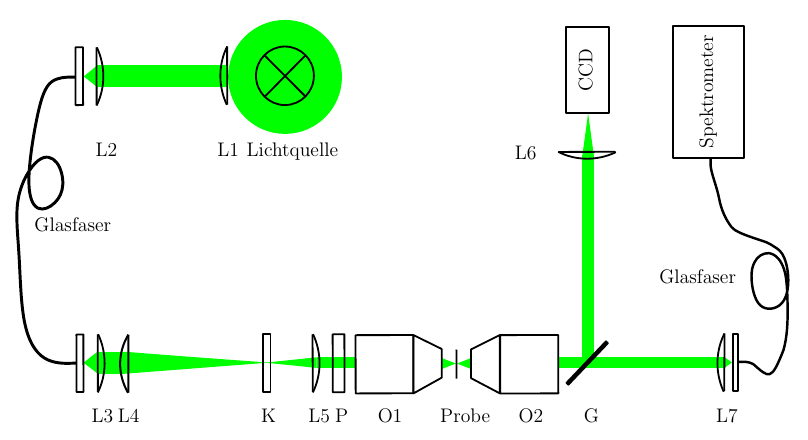
\includegraphics[width=\textwidth]{Figures/Setup.png}
      \caption{Schematic set up of all optical components.\cite{bib:Anleitung}}
      \label{fig:Setup}
    \end{figure}
    \newline
    \begin{minipage}{0.41\textwidth}
      \begin{description}
        \item[L1:] Lens($\SI{-100}{\milli\meter}$)
        \item[L2:] Lens($\SI{+25.4}{\milli\meter}$) on 3D table
        \item[L3:] Lens($\SI{-40}{\milli\meter}$)
        \item[L4:] Lens($\SI{+200}{\milli\meter}$)
        \item[L5:] Lens($\SI{-50}{\milli\meter}$)
        \item[L6:] Lens($\SI{+50}{\milli\meter}$)
        \item[L7:] Lens($\SI{+40}{\milli\meter}$) on 3D table
      \end{description}
    \end{minipage}\quad
    \begin{minipage}{0.55\textwidth}
      \begin{description}
        \item[G:] Angled glass plate
        \item[K:] Double-Knife-Edge
        \item[O1:] First objective(+) static
        \item[O2:] Second objective(-) on 3D table
        \item[P:] Polarisation plate
        \item[Probe:] Sheet of glass with samples on it on 3D table
      \end{description}
    \end{minipage}
    
    \newpage
    %%%%%%%%%%%%%%%%%%%%%%%%%%%%%%
    %%%%%%%%%%%%%%%%%%%%%%%%%%%%%%
    %%%%%%%%%%%%%%%%%%%%%%%%%%%%%%
    \begin{section}{Adjusting the optical path}
      \label{chp:SetupOptics}
      To set up this experiment we started by aligning the light source to be
      parallel to the edges of our work plate and fixed it at a moderate height.
      Directly behind the light source in the optical path, we placed a lens
      with a focal length of $\SI{-100}{\milli\meter}$. \newline
      From here on we will describe a lens and its orientation in the form of
      \textbf{lens($\pm \SI{100}{\milli\meter}$)} where the number
      represents the focal length and the provided sign the orientation in
      relation to the optical path. $-$ being the case, that the focal point is
      in the optical path but \textbf{in front} of the lens pointing towards the
      source of light. And $+$ being the opposite case of the focal point being
      \textbf{behind} the lens i.e. further away from the light source. \newline
      With the first lens placed roughly inside the path, we adjust the height
      of the beam by following it with a sharply pointed cone so that the middle
      of the beam is always the same height as the height-fixed cone.
      After the first lens is adjusted and fixed, we placed the second 
      lens($\SI{+25.4}{\milli\meter}$) mounted on a 3D movable table in the beam
      and roughly adjust its height with the pre-fixed cone.
      Now, the beam has to be focused into a glass fibre, which we placed
      directly behind the lens($\SI{+25.4}{\milli\meter}$) and adjust its height
      to be in the middle of the beam. Continuing the beam as shown in
      \cref{fig:Setup} we placed a lens($\SI{-40}{\milli\meter}$) behind the
      other end of the glass fibre and another lens($\SI{+200}{\milli\meter}$)
      behind that. Their height is calibrated using the cone and their position
      is adjusted so that their focal point is as sharp as possible and on the
      correct height.
      A double knife edge is placed directly in this focal point.\newline
      Following the knife edge we placed a lens($\SI{-50}{\milli\meter}$) to
      collimate the beam into a polarisation plate we that we placed behind the
      lens. Both their heights are adjusted with the cone yet again.
      Now we placed the first objective(+) in the beam and fix it at the correct
      height. After the first objective(+) we placed the sample and the second
      objective(-), which were both mounted on 3D tables. At this point we
      painfully noticed, that, because of the layout we chose, we did not have
      enough space on the work plate to fix every component properly and also
      that we chose a height at which we did not have enough travel distance
      with the 3D tables to fully reach every part of the sample plate and
      adjust the beam correctly. Because of this initial design flaw we had to
      start over adjusting everything again to accommodate the limited
      travel distances of the 3D tables. \newline
      After we finished this and reached this point again, we placed a glass
      plate in the beam behind the second objective(-) and angled it to
      reflect a part of the beam into a CCD camera. In the part of the beam
      to the camera, we placed a lens($\SI{+50}{\milli\meter}$) to focus the
      beam onto the camera chip. After adjusting the heights this beam branch
      was fixed.\newline
      In the other branch that was transmitted through the glass plate, we
      placed the last lens($\SI{+40}{\milli\meter}$) which was mounted on
      another 3D table. After its height had been roughly adjusted we placed
      another glass fibre behind it and connected its other end to the
      spectrometer. \newline
      At this point the building of the optical path was completed
      and we started calibrating the beam. To do so, we optimized the intensity
      received by the spectrometer by adjusting the
      lens($\SI{+25.4}{\milli\meter}$) and the lens($\SI{+40}{\milli\meter}$)
      on their 3D tables to focus the light as good as possible into the glass
      fibres. After the intensity has been optimized, we adjusted both the
      double knife edge and the second objective(-) to project the knife edge
      as good as possible onto the CCD camera. To place the sample plate as good
      as possible in the focal points of the objectives, we moved the edge of
      glass in sight and adjusted this to be as sharp as possible on the CCD
      camera. \newline
      Now that the beam had been adjusted and optimized, we searched for the
      samples by moving the sample plate and placed the knife edges, so that
      only one sample was visible. \newline
      With everything configured correctly, we moved the sample plate a little
      around to learn how the samples were arranged and to get an idea of the
      layout and the position we were actually looking at.
      \vfill
    \end{section}
    %%%%%%%%%%%%%%%%%%%%%%%%%%%%%
    
    
    
    %%%%%%%%%%%%%%%%%%%%%%%%%%%%%%
    %%%%%%%%%%%%%%%%%%%%%%%%%%%%%%
    %%%%%%%%%%%%%%%%%%%%%%%%%%%%%%
    \begin{section}{Taking measurements}
      \label{chp:SetupMeasuring}
      To start the actually collection of measurements we confirmed our starting
      position and mapped out a pattern by which we would go through all
      samples. Throughout the entire measuring phase, we often confirmed our
      current whereabouts on the sample plate to not confuse the measurements.
      Having established a pattern by which we would proceed, we adjusted the
      polarisation plate to be at an angle of $\SI{0}{\degree}$ and also
      adjusted the intensity of the light source so that the spectrometer was
      not reaching its saturation. \newline
      With everything now set up correctly we blocked the beam to measure the
      first \textit{Dark-Spectrum}. We proceeded with taking measurements and
      taking \textit{Reference-Spectra} at the beginning and after every two
      samples we measured. When taking the \textit{Reference-Spectra}, we also
      checked if the sensor was reaching saturation. \newline
      We applied the same procedure to the measurements taken with the
      polarisation plate set at $\SI{0}{\degree}$.
      
      \begin{table}[htbp]
        \centering
        \begin{tabular}{|c|c|c|c|c|c|}
          \hline
          \multirow{2}{*}{Row} & \multicolumn{5}{|c|}{Sample columns} 
          \\ \cline{2-6}
          & $A /\SI{}{\nano\meter}$ & $B /\SI{}{\nano\meter}$ &
          $C /\SI{}{\nano\meter}$ & $D /\SI{}{\nano\meter}$ &
          $E /\SI{}{\nano\meter}$\\ \hline \hline 
          1 & 140 & 250 & 300 & 150 & 100 \\ \hline 
          2 & 170 & 275 & 325 & 160 & 120 \\ \hline 
          3 & 200 & 300 & 350 & 170 & 140 \\ \hline 
          4 & 230 & 325 & 375 & 180 & 160 \\ \hline 
          5 &  & 350 & 400 & 190 & 180 \\ \hline 
          6 &  & 375 & 425 &  & 200 \\ \hline 
          7 &  & 400 & 450 &  & 220 \\ \hline 
          8 &  & 425 & 475 &  & 240 \\ \hline 
          9 &  & 450 & 500 &  &  \\ \hline 
        \end{tabular}
        \caption{Pattern of samples on the glass plate.}
        \label{tab:samplepattern}
      \end{table}
      
      \todo[inline]{hier noch mehr zu den samples schreiben. vielleich ein 
      description ding machen.}
      
    \end{section}
    %%%%%%%%%%%%%%%%%%%%%%%%%%%%%
    
  \end{chapter}
  %%%%%%%%%%%%%%%%%%%%
  
  
  
  %%%%%%%%%%%%%%%%%%%%
  %%%%%%%%%%%%%%%%%%%%
  %%%%%%%%%%%%%%%%%%%%
  \begin{chapter}{Analysis of the data}
    \label{chp:Analysis}
    When analysing the spectra, we have to subtract the dark spectrum from
    all reference spectra to correct for any background light in the
    measurements.
    To analyse any recorded transmission spectrum, we plot the transmission
    spectra through a nano structure as percentage of the reference spectrum
    through glass alone without any nano structure.
    This is all done automatically by the software used in this experiment.
    Since we will mostly look for an minimum of transmission in the spectra,
    we show any plotted data series with a negative Gaussian function already
    fitted. We use \cref{eq:TransspecFitting} as form of functions to be fitted
    to our data. For this equation, \textit{a, m} and \textit{$\sigma$} will be
    it's degrees of freedom.
    \begin{equation}
      \label{eq:TransspecFitting}
      f(x)=100-a\cdot exp\left(-\left(\frac{x-m}{\sqrt{2}\cdot\sigma}
      \right)^{2}\right)
    \end{equation}
    The distorted an noisy data points at the beginning and the end of the
    will be ignored by us and are probably an effect of differing accuracy
    of counts within the spectrum  of the devices used by us.
    Perhaps the spectrometer is only most accurate in the range from
    $\SI{500}{\nano\meter}$ up to about $\SI{950}{\nano\meter}$ wavelengths.
    This hypothesis is backed up by the reference spectra we took 
    (\cref{Appendix:Data}).
    In those it is clear, that below a wavelength of $\SI{500}{\nano\meter}$
    and beyond one of $\SI{850}{\nano\meter}$, the number of counts through
    mere glass drops dramatically and well below of about $750$ counts per
    integrated measurement. This small amount of events seems to not be enough
    to provide a valid and accurate measure of transmission percentage.
    Because of this,  we limit the range of values used to fit the negative
    Gaussian function to a much smaller area to stabilize the fitting process.
    The fitted function is therefore only shown inside the range of values
    actually used to fit the function. \newline
    Additionally, it has to be said, that no data series has been changed by us
    in the process of making this Report. The uncertainties for every fit
    parameters are provided by the fitting software used.
    In this case, we used \textit{PYTHON} and the \textit{curve\_fit} function
    from \textit{scipy.optimize}.
    To make the development of each transmission minimum and it's location more
    easy to follow, we plotted them with regard to the varying parameter for
    each sample column. And to further illustrate any potential relations, we
    then added a fitted curve to those minima positions.
    For columns \textbf{A}, \textbf{D} and \textbf{E} it was obvious to use a
    straight line, so we used a function with \cref{eq:gerade} as general form.
    \begin{equation}
      \label{eq:gerade}
      f(d) = m\cdot d + n
    \end{equation}
    For column \textbf{B} we used a function with \cref{eq:oneoverrsq} as
    general form.
    \begin{equation}
      \label{eq:oneoverrsq}
      f(r) = \frac{a}{r^{2}}+b
    \end{equation}
    And finally for column \textbf{C} we used a second degree polynomial
    function with \cref{eq:parabola} as general form.
    \begin{equation}
      \label{eq:parabola}
      f(x) = a\cdot x^{2} + b\cdot x + c
    \end{equation}
    
    
    
    %%%%%%%%%%%%%%%%%%%%%%%%%%%%%%
    %%%%%%%%%%%%%%%%%%%%%%%%%%%%%%
    %%%%%%%%%%%%%%%%%%%%%%%%%%%%%%
    \begin{section}{Column \textbf{A}: Disks with variable diameters}
      \label{chp:DataA}
      Column \textbf{A} contains four structures of simple disks in a constant
      lattice of $\SI{400}{\nano\meter}$ but varying the diameter of the disks
      in for each structure. The recorded transmission spectra can be found in
      \cref{fig:TransspecFIT_APol0,fig:TransspecFIT_APol90}.
      In those graphics, one can observe how the resonating frequency of the
      structures change through the positions of their transmission minima.
      For larger diameters of disks, the resonating frequency shifts towards
      higher wavelengths and the blockage percentage increases.
      This effect is observable in the measurements for $\SI{0}{\degree}$ as
      well as for $\SI{90}{\degree}$ polarisation. The relation between the
      changed parameter and the resulting change of resonant frequency seems to
      be linear, so we fitted a linear function to the positions development.
      This linear relation (\cref{fig:MinimaPosA}) is expected by the
      semi-classical model, since the symmetrically and linear growing disks
      allow for a equally linear growing resonating wavelength. Since the
      disks are supposed to be round and symmetrical, we would also expect the
      two slopes to be equal, which we found not to be true with our
      measurements. But where a mutual slope is still within both ranges of
      error, we would also expect not this kind of offset between the two
      polarisations. In the semi-classical model we would expect both linear
      developments to be about the same. We can therefore only suspect, that
      some other factor involved might have changed the outcome of our
      measurements. Maybe the disks might be of equal size and shape, but the
      shape of the lattice they are arranged in differs in both directions.
      Or it could be due to some kind of refraction effect along the optical
      path, which could shift the wavelengths to higher or lower values.
      \todo[inline]{letzten 2 sätze: richtig so?}
      
      \todo[inline]{Fertig???}
      
      \begin{figure}[b!]
        \centering
        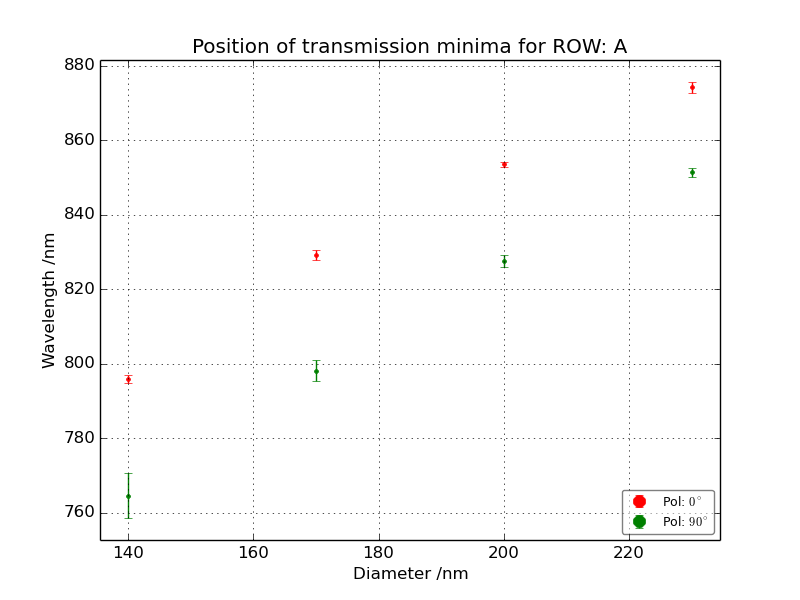
\includegraphics[width=\textwidth]{Figures/MinimaPosA.png}
        \caption{Wavelength positions of the transmission minima for column
            \textbf{A}.}
        \label{fig:MinimaPosA}
      \end{figure}
      \newpage
      \begin{figure}[ht!]
        \centering
        \begin{minipage}{.95\textwidth}
          \centering
          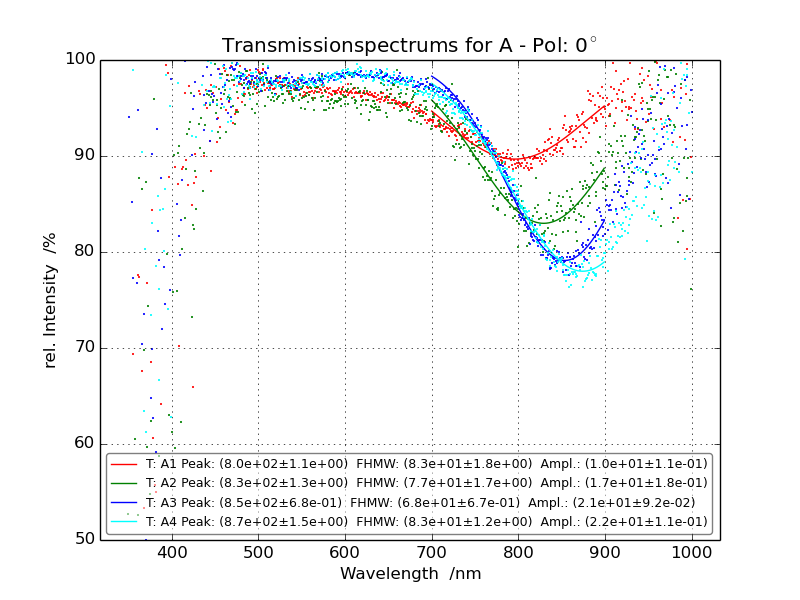
\includegraphics[width=\textwidth]
              {Figures/TransspecFIT_APol0.png}
          \caption{Data for sample-column \textbf{A} at $\SI{0}{\degree}$
              polarisation with fitted Gaussian function.}
          \label{fig:TransspecFIT_APol0}
        \end{minipage}\\
        \begin{minipage}{.95\textwidth}
          \centering
          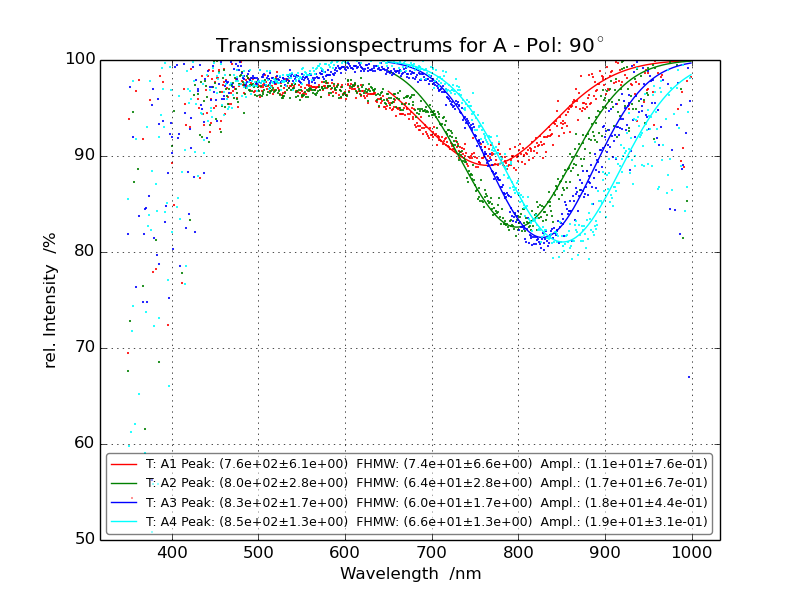
\includegraphics[width=\textwidth]
              {Figures/TransspecFIT_APol90.png}
          \caption{Data for sample-column \textbf{A} at $\SI{90}{\degree}$
              polarisation with fitted Gaussian function.}
          \label{fig:TransspecFIT_APol90}
        \end{minipage}
      \end{figure}
      
    \end{section}
    %%%%%%%%%%%%%%%%%%%%%%%%%%%%%%
    
    
    
    \newpage
    %%%%%%%%%%%%%%%%%%%%%%%%%%%%%%
    %%%%%%%%%%%%%%%%%%%%%%%%%%%%%%
    %%%%%%%%%%%%%%%%%%%%%%%%%%%%%%
    \begin{section}{Column \textbf{B}: Dimers with variable Mid-to-Mid
        distances}
      \label{chp:DataB}
      Column \textbf{B} contains nine structures of Dimers with constant
      diameters of $\SI{200}{\nano\meter}$ and lattice of
      $\SI{670}{\nano\meter}$ Mid-to-Mid but varying Mid-to-Mid positions. From
      \cref{fig:TransspecFIT_BPol0,fig:TransspecFIT_BPol90}, it possible to see
      different responses of the resonant frequency for two different
      polarisations. In the case of $\SI{0}{\degree}$ polarisation, the
      resonating wavelengths are shifted to smaller values with a growing
      Mid-to-Mid distance in the Dimers. Furthermore, the distance of each
      shift decreases with every step of increased Mid-to-Mid distance.
      For the $\SI{90}{\degree}$ polarisation the resonating frequency shifts
      in the other direction, but it is still decreasing with every sample.
      There is however, a difference in blocked intensity for both
      polarisations. Whereas all transmission values at $\SI{0}{\degree}$
      polarisation are below $\SI{60}{\percent}$ the transmitted intensity
      at $\SI{90}{\degree}$ polarisation is between $\SI{60}{\percent}$ and 
      $\SI{70}{\percent}$.\newline
      The semi-classical model predicts for this experiment a relation of the
      form of \cref{eq:oneoverrsq}. Fitting a curve of this form we notice,
      that this kind of relation describes our data very good for both
      polarisations. Only the first data point of $\SI{0}{\degree}$ polarisation
      seems to be a little off. Fitting the function without this measurement,
      the curve describes the progression even better.
      
      \todo[inline]{Fertig???}
      
      \begin{figure}[b!]
        \centering
        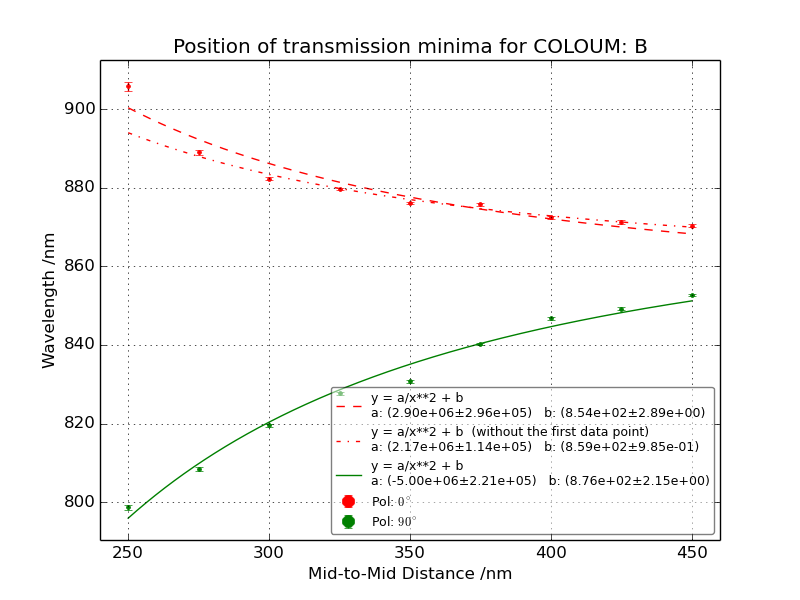
\includegraphics[width=\textwidth]{Figures/MinimaPosB.png}
        \caption{Wavelength positions of the transmission minima for column
            \textbf{B}.}
        \label{fig:MinimaPosB}
      \end{figure}
      \newpage
      \begin{figure}[ht!]
        \centering
        \begin{minipage}{.95\textwidth}
          \centering
          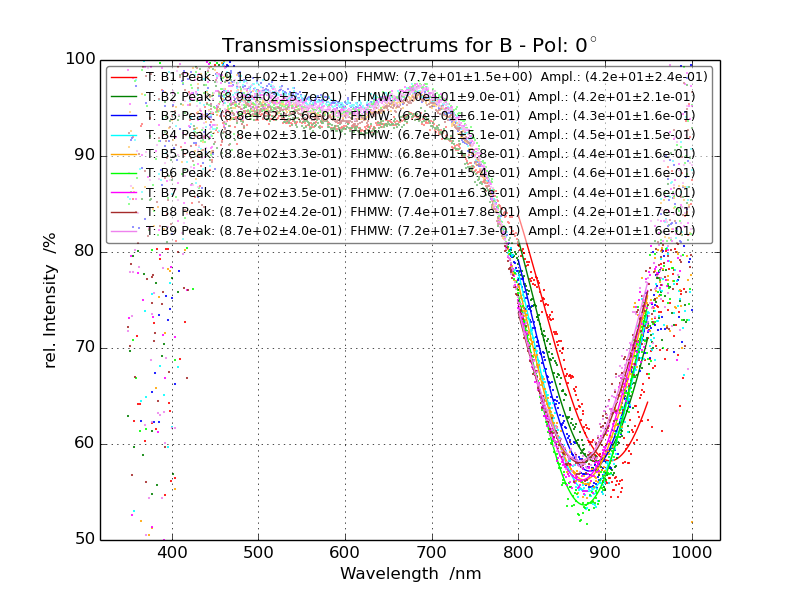
\includegraphics[width=\textwidth]
              {Figures/TransspecFIT_BPol0.png}
          \caption{Data for sample-column \textbf{B} at $\SI{0}{\degree}$
              polarisation with fitted Gaussian function.}
          \label{fig:TransspecFIT_BPol0}
        \end{minipage}\\
        \begin{minipage}{.95\textwidth}
          \centering
          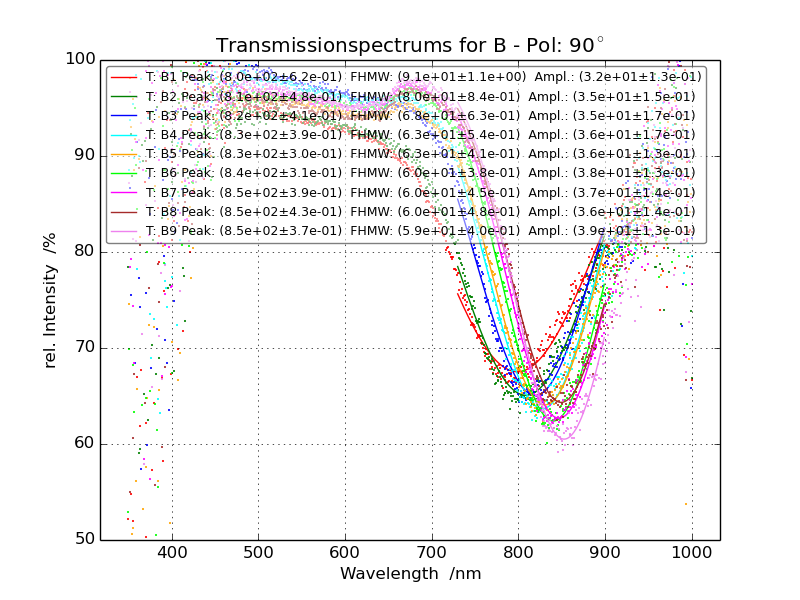
\includegraphics[width=\textwidth]
              {Figures/TransspecFIT_BPol90.png}
          \caption{Data for sample-column \textbf{B} at $\SI{90}{\degree}$
              polarisation with fitted Gaussian function.}
          \label{fig:TransspecFIT_BPol90}
        \end{minipage}
      \end{figure}
      
    \end{section}
    %%%%%%%%%%%%%%%%%%%%%%%%%%%%%%
    
    
    
    \newpage
    %%%%%%%%%%%%%%%%%%%%%%%%%%%%%%
    %%%%%%%%%%%%%%%%%%%%%%%%%%%%%%
    %%%%%%%%%%%%%%%%%%%%%%%%%%%%%%
    \begin{section}{Column \textbf{C}: Disks with variable period}
      \label{chp:DataC}
      Column \textbf{C} contains nine structures of Dimers with constant
      diameters of $\SI{200}{\nano\meter}$ but this time varying period
      Mid-to-Mid distances.
      From looking at the plotted spectra, it is not very obvious to see any
      pattern other than a change in transmitted intensity.
      Plotting positions of the transmission minima, it is much easier to
      observe some kind of relation between the changed parameters.\newline
      Theory predicts 
      \todo[inline]{What exactly???}
      
      \begin{figure}[b!]
        \centering
        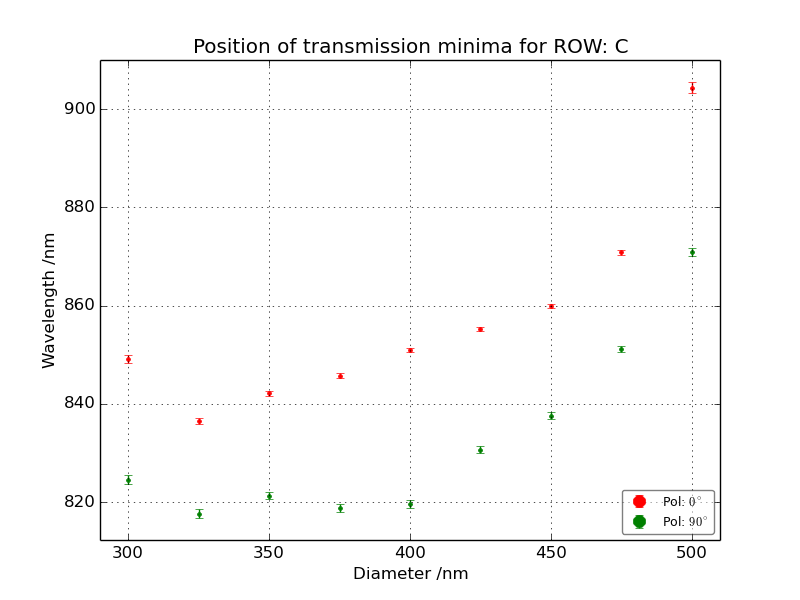
\includegraphics[width=\textwidth]{Figures/MinimaPosC.png}
        \caption{Wavelength positions of the transmission minima for column
            \textbf{C}.}
        \label{fig:MinimaPosC}
      \end{figure}
      \newpage
      \begin{figure}[ht!]
        \centering
        \begin{minipage}{.95\textwidth}
          \centering
          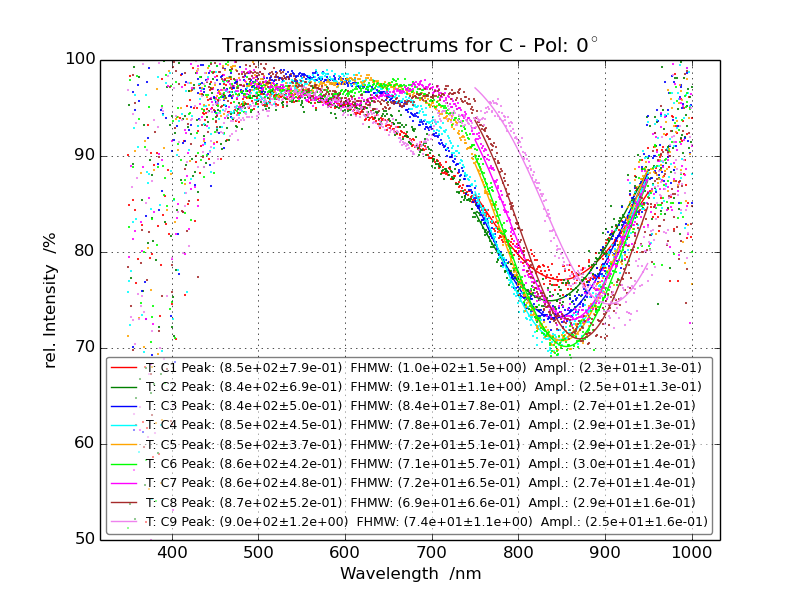
\includegraphics[width=\textwidth]
              {Figures/TransspecFIT_CPol0.png}
          \caption{Data for sample-column \textbf{C} at $\SI{0}{\degree}$
              polarisation with fitted Gaussian function.}
          \label{fig:TransspecFIT_CPol0}
        \end{minipage}\\
        \begin{minipage}{.95\textwidth}
          \centering
          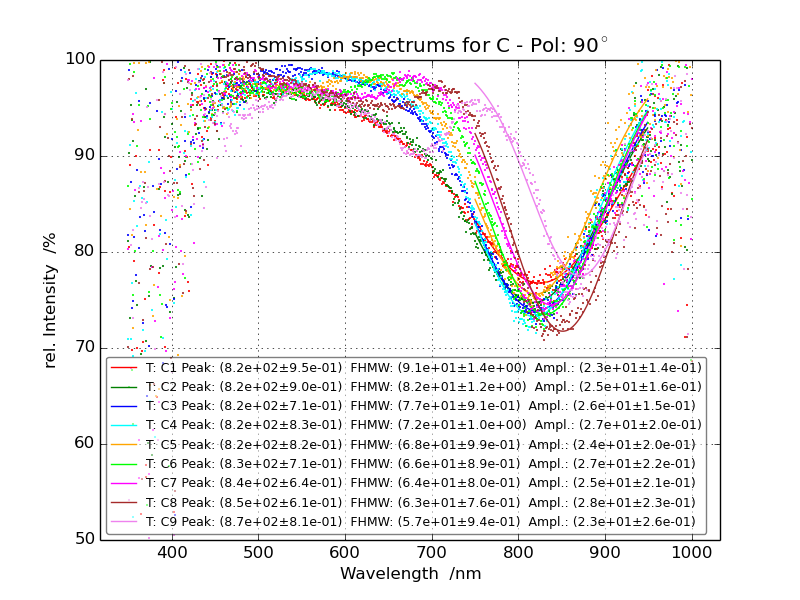
\includegraphics[width=\textwidth]
              {Figures/TransspecFIT_CPol90.png}
          \caption{Data for sample-column \textbf{C} at $\SI{90}{\degree}$
              polarisation with fitted Gaussian function.}
          \label{fig:TransspecFIT_CPol90}
        \end{minipage}
      \end{figure}
      
    \end{section}
    %%%%%%%%%%%%%%%%%%%%%%%%%%%%%%
    
    
    
    \newpage
    %%%%%%%%%%%%%%%%%%%%%%%%%%%%%%
    %%%%%%%%%%%%%%%%%%%%%%%%%%%%%%
    %%%%%%%%%%%%%%%%%%%%%%%%%%%%%%
    \begin{section}{Column \textbf{D}: Pentamers with variable Mid-to-Mid
        distances}
      \label{chp:DataD}
      Column \textbf{D} contains five structures of Pentamers with a constant
      lattice of $\SI{900}{\nano\meter}$ and disk diameter of
      $\SI{140}{\nano\meter}$ but varying Mid-Disk-to-Mid-Disk distances.
      Again, only by looking at the measured spectra it is very difficult to
      make out any kind of relation between the Mid-Disk-to-Mid-Disk distances
      and the position of the transmission minima. Fitting the negative Gaussian
      functions and plotting their dip positions however is far more revealing.
      Except for the first data point in the $\SI{0}{\degree}$ polarisation
      series and the third data point in the $\SI{90}{\degree}$ series, both
      sample columns follow a linear progression. This is exactly what the
      theory predicts for this case. Due to the symmetry of the Pentamers and
      the symmetrical changes applied to them, their resonant frequency
      responses similar to the resonance of a single disk. \newline
      The two points that do not follow this linear function are probably a
      result of some kind of instability during the fitting operation and not
      of much relevance.\newline
      Just like in \cref{chp:DataA} both slopes should be about the same and
      they do match with both their ranges of error. But exactly like before in
      \cref{chp:DataA}, their appears to be some kind of effect which offsets
      both linear progressions only this time by about half the distance it
      was set off in \cref{chp:DataA}.
      
      \todo[inline]{Fertig???}
      
      \begin{figure}[b!]
        \centering
        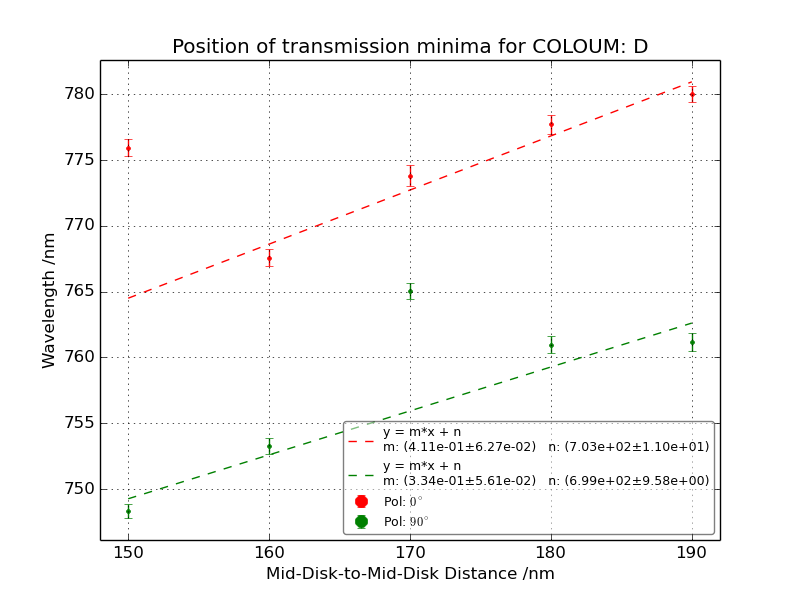
\includegraphics[width=\textwidth]{Figures/MinimaPosD.png}
        \caption{Wavelength positions of the transmission minima for column
            \textbf{D}.}
        \label{fig:MinimaPosD}
      \end{figure}
      \newpage
      \begin{figure}[ht!]
        \centering
        \begin{minipage}{.95\textwidth}
          \centering
          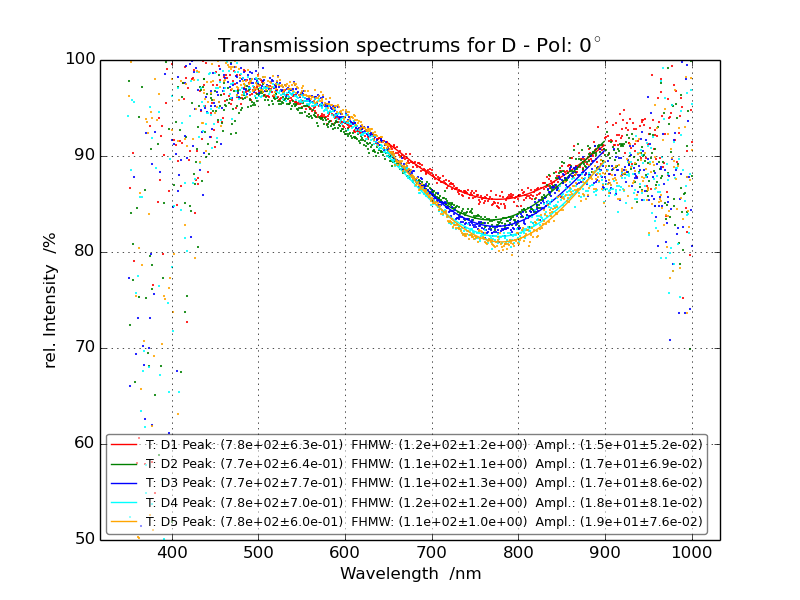
\includegraphics[width=\textwidth]
              {Figures/TransspecFIT_DPol0.png}
          \caption{Data for sample-column \textbf{D} at $\SI{0}{\degree}$
              polarisation with fitted Gaussian function.}
          \label{fig:TransspecFIT_DPol0}
        \end{minipage}\\
        \begin{minipage}{.95\textwidth}
          \centering
          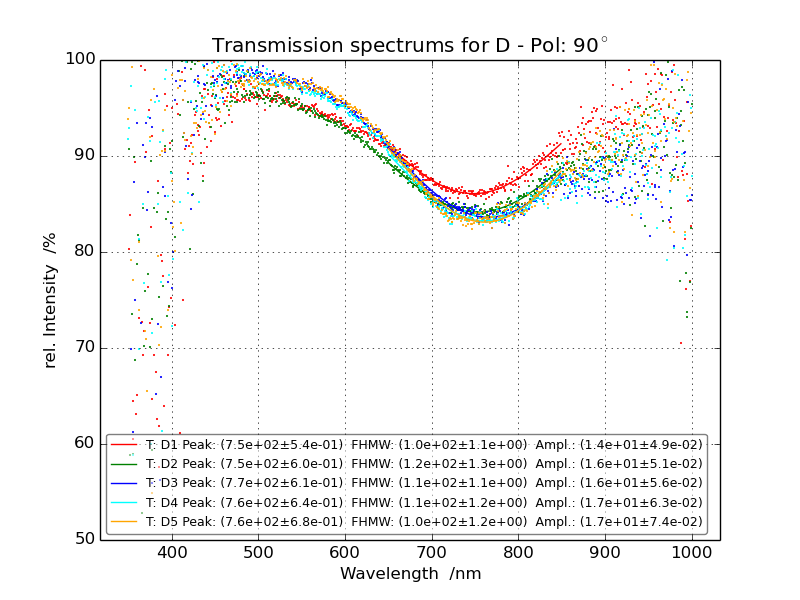
\includegraphics[width=\textwidth]
              {Figures/TransspecFIT_DPol90.png}
          \caption{Data for sample-column \textbf{D} at $\SI{90}{\degree}$
              polarisation with fitted Gaussian function.}
          \label{fig:TransspecFIT_DPol90}
        \end{minipage}
      \end{figure}
      
    \end{section}
    %%%%%%%%%%%%%%%%%%%%%%%%%%%%%%
    
    
    
    \newpage
    %%%%%%%%%%%%%%%%%%%%%%%%%%%%%%
    %%%%%%%%%%%%%%%%%%%%%%%%%%%%%%
    %%%%%%%%%%%%%%%%%%%%%%%%%%%%%%
    \begin{section}{Column \textbf{E}: Ellipses with variable length of
        major axis}
      \label{chp:DataE}
      Column \textbf{E} contains eight structures of Ellipses with a constant
      lattice of $\SI{750}{\nano\meter}$ and disk diameter
      $\delta_{x} = \SI{140}{\nano\meter}$ but varying disk diameter
      $\delta_{y}$.
      
      \todo[inline]{Written analysis here!}
      
      \begin{figure}[b!]
        \centering
        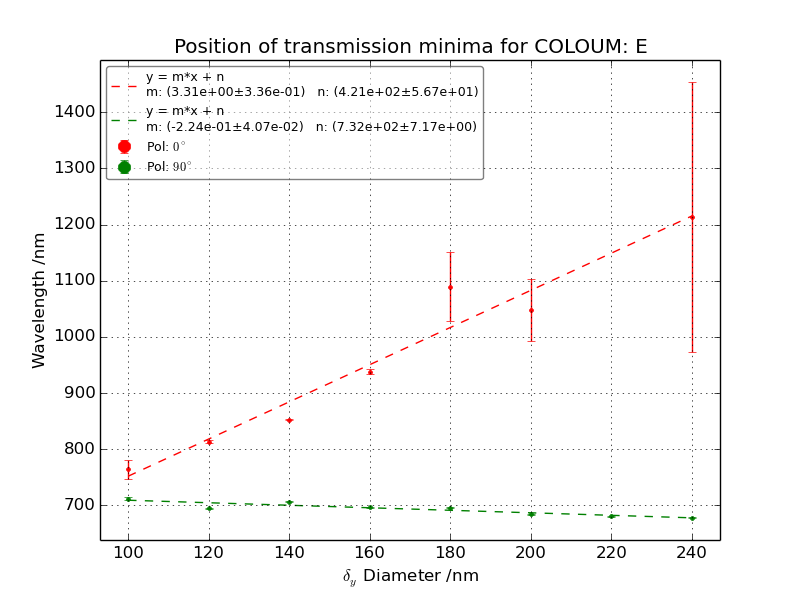
\includegraphics[width=\textwidth]{Figures/MinimaPosE.png}
        \caption{Wavelength positions of the transmission minima for column
            \textbf{E}.}
        \label{fig:MinimaPosE}
      \end{figure}
      \newpage
      \begin{figure}[ht!]
        \centering
        \begin{minipage}{.95\textwidth}
          \centering
          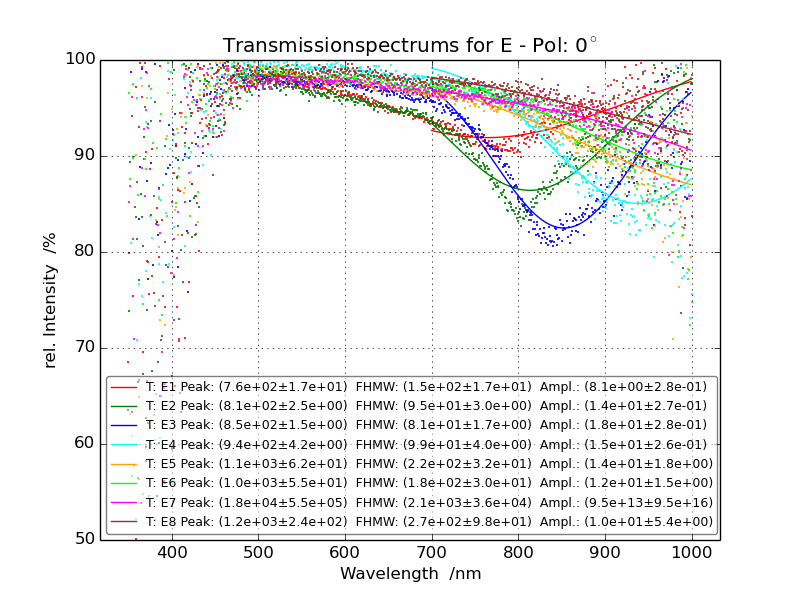
\includegraphics[width=\textwidth]
              {Figures/TransspecFIT_EPol0.png}
          \caption{Data for sample-column \textbf{E} at $\SI{0}{\degree}$
              polarisation with fitted Gaussian function.}
          \label{fig:TransspecFIT_EPol0}
        \end{minipage}\\
        \begin{minipage}{.95\textwidth}
          \centering
          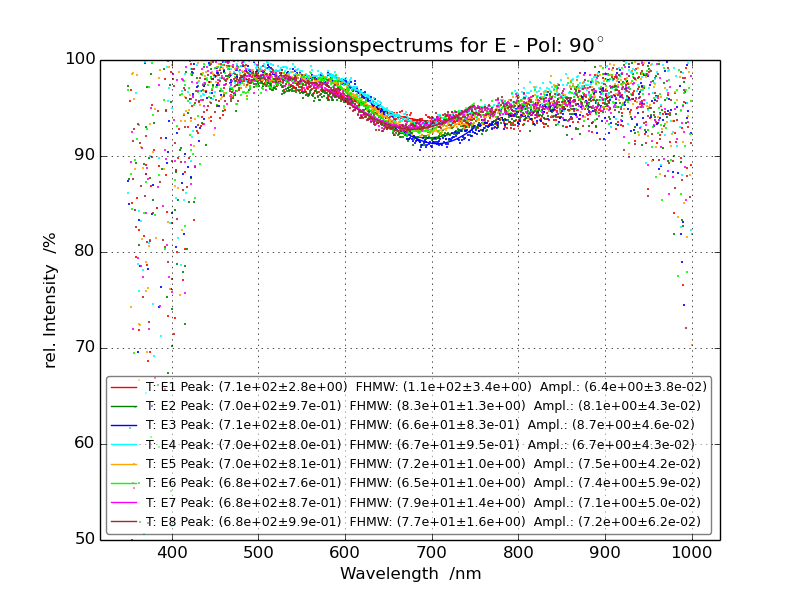
\includegraphics[width=\textwidth]
              {Figures/TransspecFIT_EPol90.png}
          \caption{Data for sample-column \textbf{E} at $\SI{90}{\degree}$
              polarisation with fitted Gaussian function.}
          \label{fig:TransspecFIT_EPol90}
        \end{minipage}
      \end{figure}
      
    \end{section}
    %%%%%%%%%%%%%%%%%%%%%%%%%%%%%%
    
    
    
    %%%%%%%%%%%%%%%%%%%%%%%%%%%%%%
    %%%%%%%%%%%%%%%%%%%%%%%%%%%%%%
    %%%%%%%%%%%%%%%%%%%%%%%%%%%%%%
    \begin{section}{Summary}
      \label{chp:AnalysisSummary}
      
      
      
    \end{section}
    %%%%%%%%%%%%%%%%%%%%%%%%%%%%%%
   
  \end{chapter}
  %%%%%%%%%%%%%%%%%%%%
  
  
  
  %%%%%%%%%%%%%%%%%%%%
  %%%%%%%%%%%%%%%%%%%%
  %%%%%%%%%%%%%%%%%%%%
  %%%%%%%%%%%%%%%%%%%%
%%%%%%%%%%%%%%%%%%%%
%%%%%%%%%%%%%%%%%%%%
\begin{appendix}
  \label{Appendix}
  
  
  
  %%%%%%%%%%%%%%%%%%%%%%%%%%%%%%
  %%%%%%%%%%%%%%%%%%%%%%%%%%%%%%
  %%%%%%%%%%%%%%%%%%%%%%%%%%%%%%
  \begin{chapter}{Data}
    \label{Appendix:Data}
    
    \todo[inline]{maybe insert a table with all the fitted parameters.}
    
    \newpage
    %%%%%%%%%%%%%%%%%%%%%%%%%%%%%%
    %%%%%%%%%%%%%%%%%%%%%%%%%%%%%%
    %%%%%%%%%%%%%%%%%%%%%%%%%%%%%%
    \begin{section}{Column \textbf{A}}
      \label{Appendix:DataA}
      
      \begin{figure}[ht!]
        \centering
        \begin{minipage}{.92\textwidth}
          \centering
          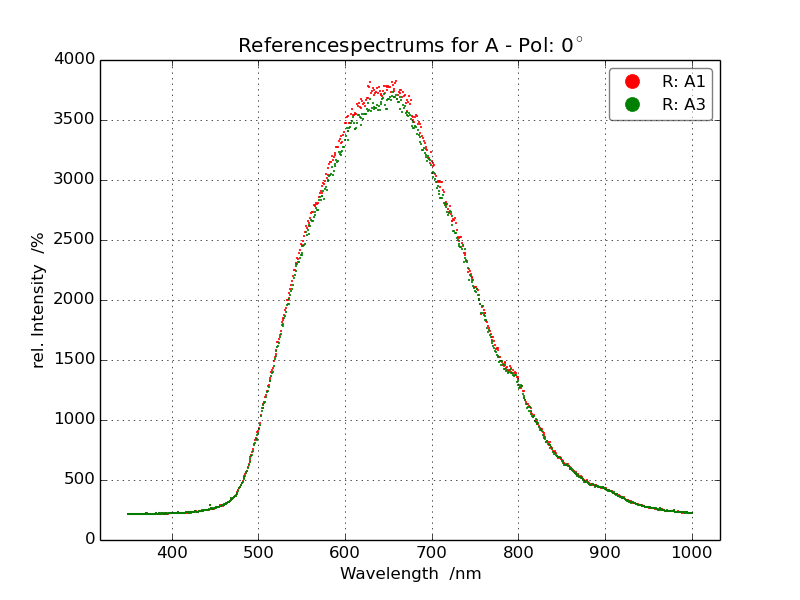
\includegraphics[width=\textwidth]{Figures/Refspec_APol0.png}
          \caption{Reference spectra for sample-column \textbf{A} at
              $\SI{0}{\degree}$ polarisation.}
          \label{fig:Refspec_APol0}
        \end{minipage}\\
        \begin{minipage}{.92\textwidth}
          \centering
          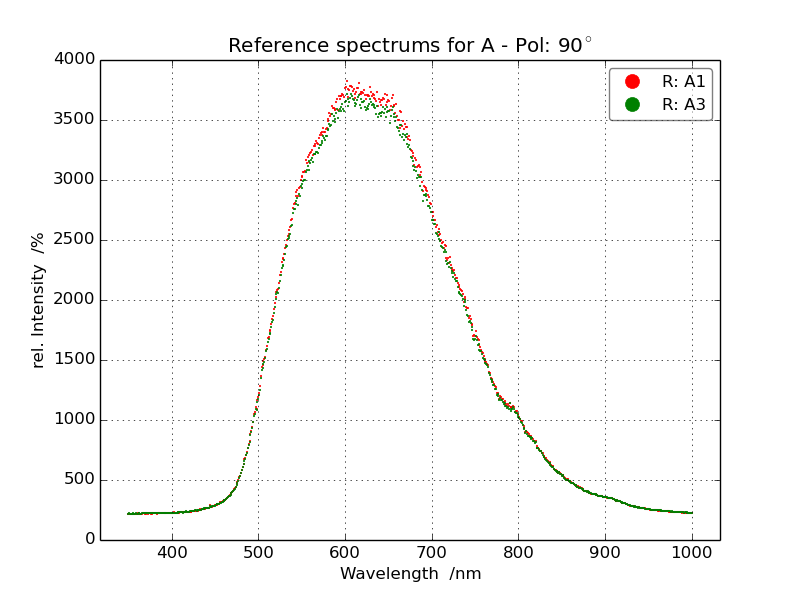
\includegraphics[width=\textwidth]{Figures/Refspec_APol90.png}
          \caption{Reference spectra for sample-column \textbf{A} at
              $\SI{90}{\degree}$ polarisation.}
          \label{fig:Refspec_APol90}
        \end{minipage}
      \end{figure}
      \newpage
      \begin{figure}[ht!]
        \centering
        \begin{minipage}{.92\textwidth}
          \centering
          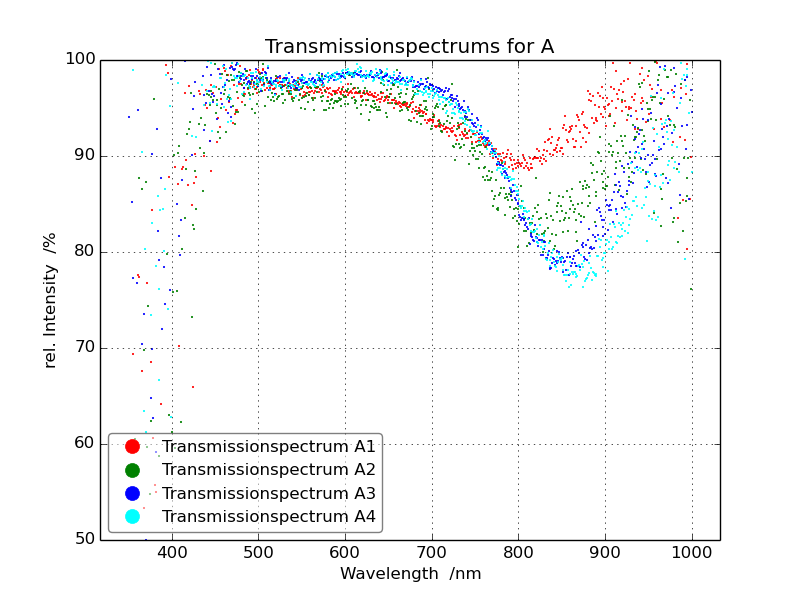
\includegraphics[width=\textwidth]{Figures/TransspecRAW_APol0.png}
          \caption{Data for sample-column \textbf{A} at $\SI{0}{\degree}$
              polarisation.}
          \label{fig:TransspecRAW_APol0}
        \end{minipage}\\
        \begin{minipage}{.92\textwidth}
          \centering
          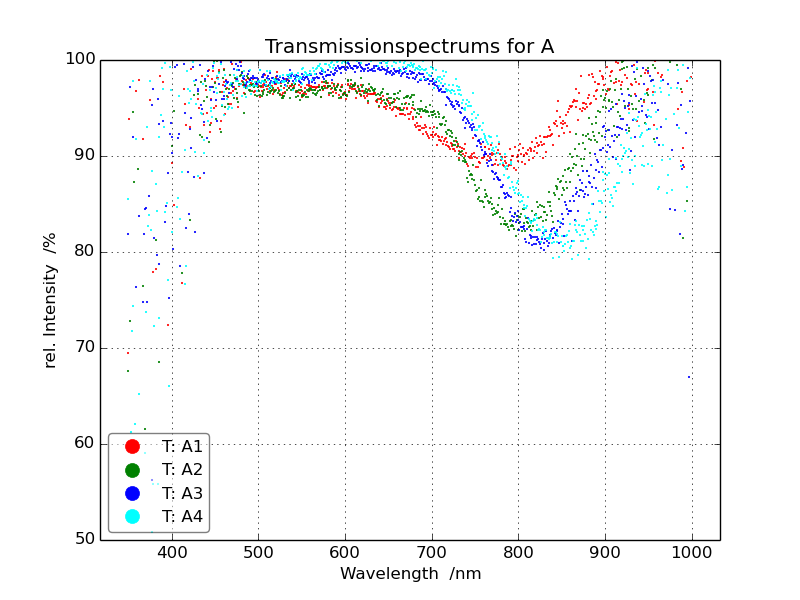
\includegraphics[width=\textwidth]{Figures/TransspecRAW_APol90.png}
          \caption{Data for sample-column \textbf{A} at $\SI{90}{\degree}$
              polarisation.}
          \label{fig:TransspecRAW_APol90}
        \end{minipage}
      \end{figure}
      
    \end{section}
    %%%%%%%%%%%%%%%%%%%%%%%%%%%%%%
    
    
    
    \newpage
    %%%%%%%%%%%%%%%%%%%%%%%%%%%%%%
    %%%%%%%%%%%%%%%%%%%%%%%%%%%%%%
    %%%%%%%%%%%%%%%%%%%%%%%%%%%%%%
    \begin{section}{Column \textbf{B}}
      \label{Appendix:DataB}
      
      \begin{figure}[ht!]
        \centering
        \begin{minipage}{.92\textwidth}
          \centering
          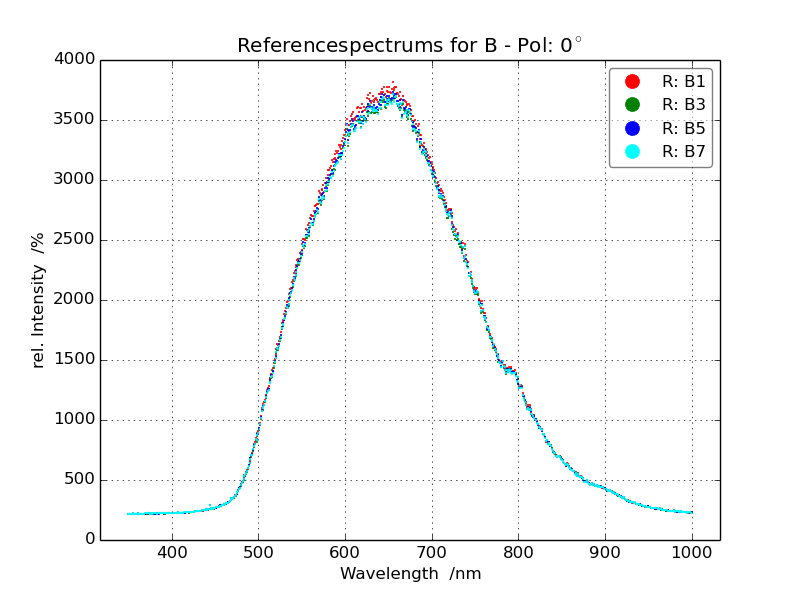
\includegraphics[width=\textwidth]{Figures/Refspec_BPol0.png}
          \caption{Reference spectra for sample-column \textbf{B} at
              $\SI{0}{\degree}$ polarisation.}
          \label{fig:Refspec_BPol0}
        \end{minipage}\\
        \begin{minipage}{.92\textwidth}
          \centering
          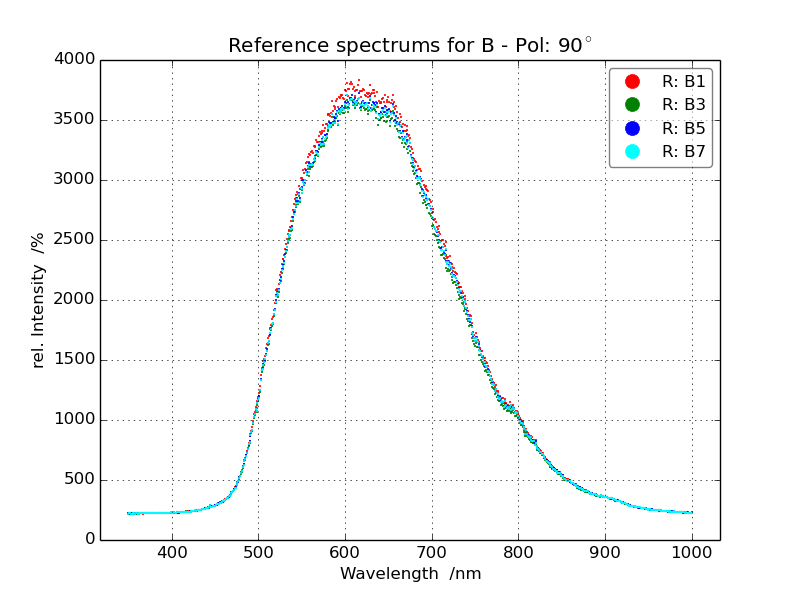
\includegraphics[width=\textwidth]{Figures/Refspec_BPol90.png}
          \caption{Reference spectra for sample-column \textbf{B} at
              $\SI{90}{\degree}$ polarisation.}
          \label{fig:Refspec_BPol90}
        \end{minipage}
      \end{figure}
      \newpage
      \begin{figure}[ht!]
        \centering
        \begin{minipage}{.92\textwidth}
          \centering
          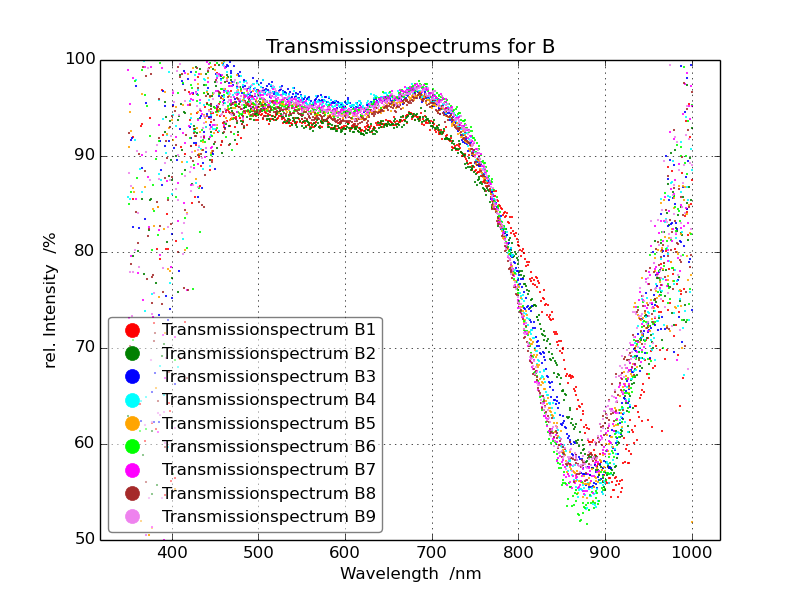
\includegraphics[width=\textwidth]{Figures/TransspecRAW_BPol0.png}
          \caption{Data for sample-column \textbf{B} at $\SI{0}{\degree}$
              polarisation.}
          \label{fig:TransspecRAW_BPol0}
        \end{minipage}\\
        \begin{minipage}{.92\textwidth}
          \centering
          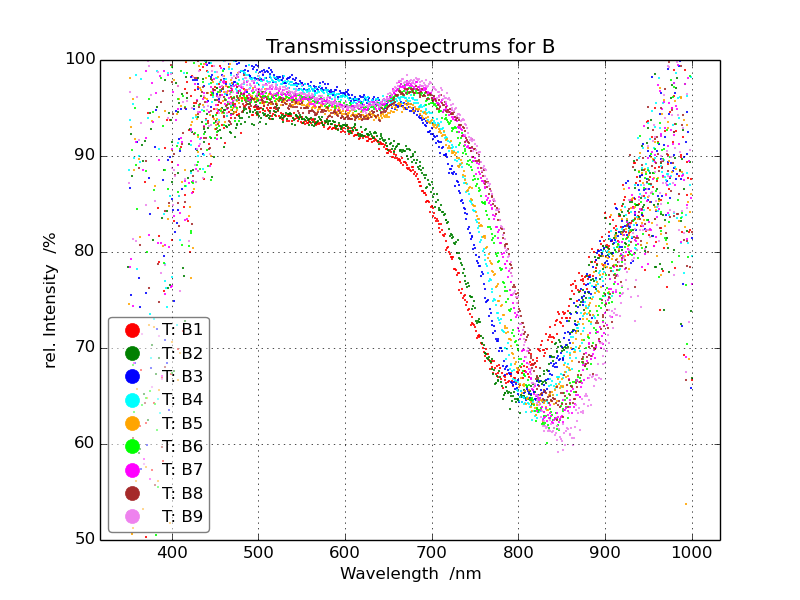
\includegraphics[width=\textwidth]{Figures/TransspecRAW_BPol90.png}
          \caption{Data for sample-column \textbf{B} at $\SI{90}{\degree}$
              polarisation.}
          \label{fig:TransspecRAW_BPol90}
        \end{minipage}
      \end{figure}
      
    \end{section}
    %%%%%%%%%%%%%%%%%%%%%%%%%%%%%%
    
    
    
    \newpage
    %%%%%%%%%%%%%%%%%%%%%%%%%%%%%%
    %%%%%%%%%%%%%%%%%%%%%%%%%%%%%%
    %%%%%%%%%%%%%%%%%%%%%%%%%%%%%%
    \begin{section}{Column \textbf{C}}
      \label{Appendix:DataC}
      
      \begin{figure}[ht!]
        \centering
        \begin{minipage}{.92\textwidth}
          \centering
          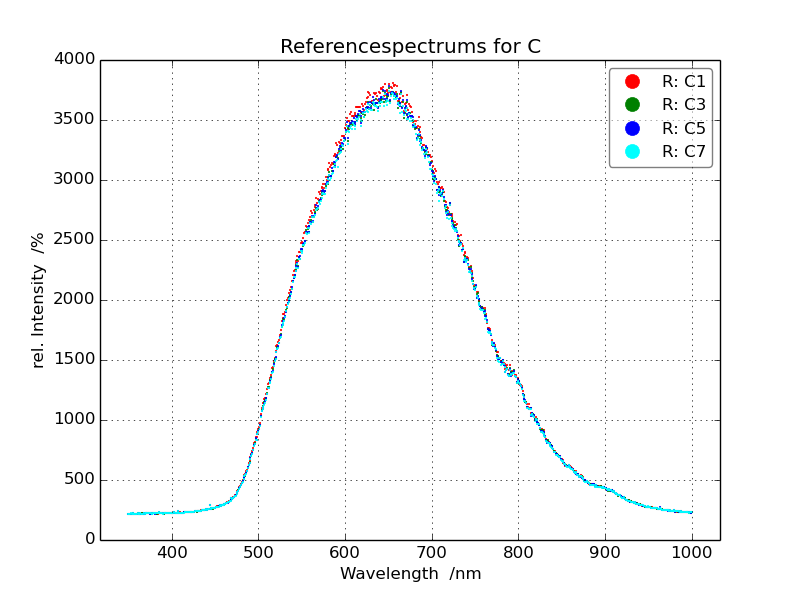
\includegraphics[width=\textwidth]{Figures/Refspec_CPol0.png}
          \caption{Reference spectra for sample-column \textbf{C} at
              $\SI{0}{\degree}$ polarisation.}
          \label{fig:Refspec_CPol0}
        \end{minipage}\\
        \begin{minipage}{.92\textwidth}
          \centering
          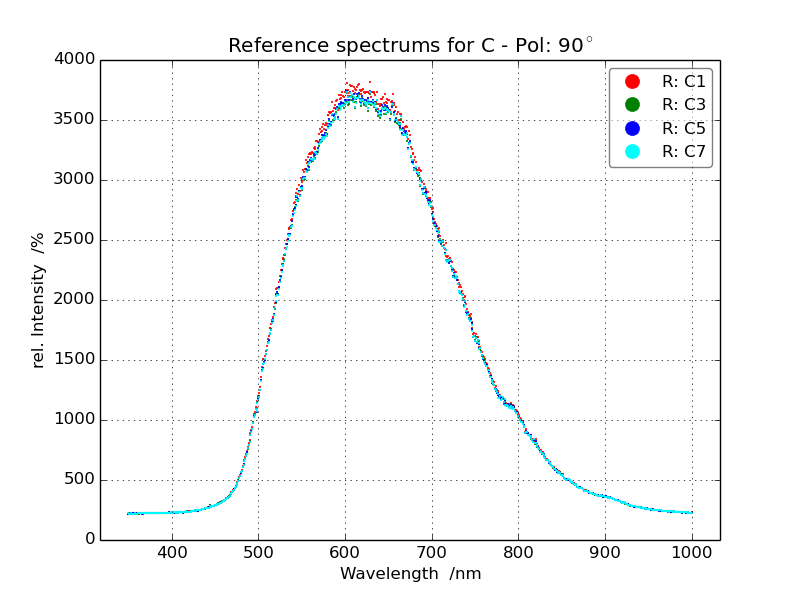
\includegraphics[width=\textwidth]{Figures/Refspec_CPol90.png}
          \caption{Reference spectra for sample-column \textbf{C} at
              $\SI{90}{\degree}$ polarisation.}
          \label{fig:Refspec_CPol90}
        \end{minipage}
      \end{figure}
      \newpage
      \begin{figure}[ht!]
        \centering
        \begin{minipage}{.92\textwidth}
          \centering
          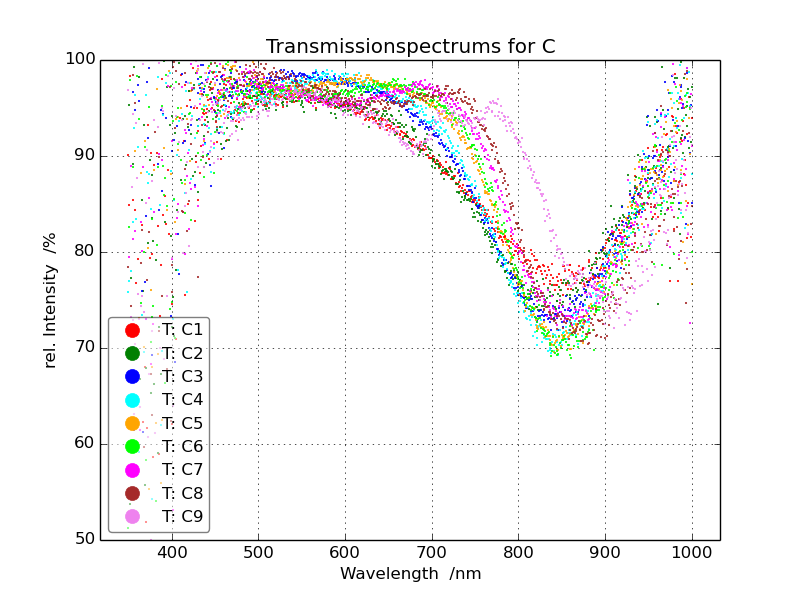
\includegraphics[width=\textwidth]{Figures/TransspecRAW_CPol0.png}
          \caption{Data for sample-column \textbf{C} at $\SI{0}{\degree}$
              polarisation.}
          \label{fig:TransspecRAW_CPol0}
        \end{minipage}\\
        \begin{minipage}{.92\textwidth}
          \centering
          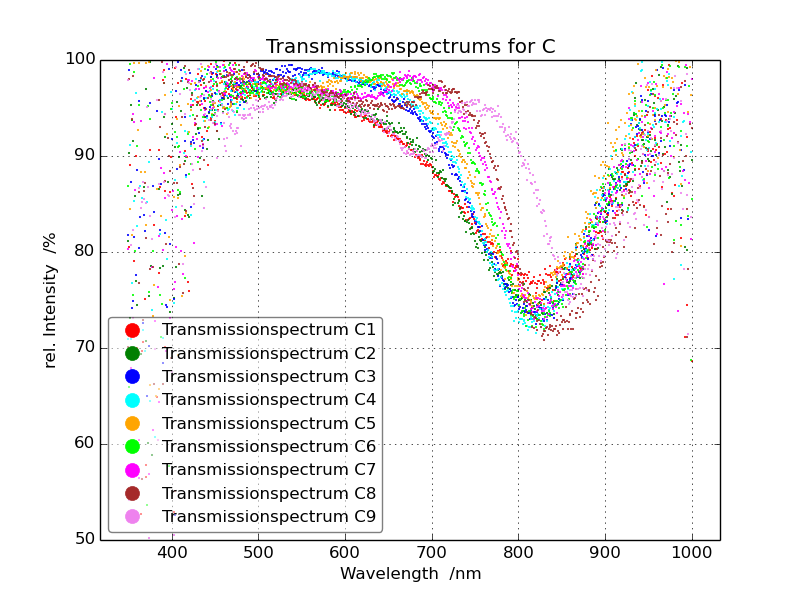
\includegraphics[width=\textwidth]{Figures/TransspecRAW_CPol90.png}
          \caption{Data for sample-column \textbf{C} at $\SI{90}{\degree}$
              polarisation.}
          \label{fig:TransspecRAW_CPol90}
        \end{minipage}
      \end{figure}
      
    \end{section}
    %%%%%%%%%%%%%%%%%%%%%%%%%%%%%%
    
    
    
    \newpage
    %%%%%%%%%%%%%%%%%%%%%%%%%%%%%%
    %%%%%%%%%%%%%%%%%%%%%%%%%%%%%%
    %%%%%%%%%%%%%%%%%%%%%%%%%%%%%%
    \begin{section}{Column \textbf{D}}
      \label{Appendix:DataD}
      
      \begin{figure}[ht!]
        \centering
        \begin{minipage}{.92\textwidth}
          \centering
          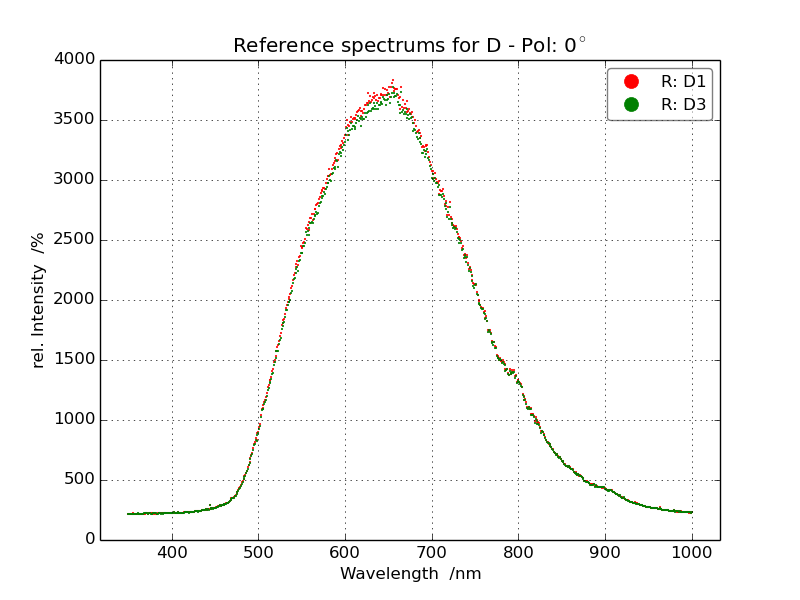
\includegraphics[width=\textwidth]{Figures/Refspec_DPol0.png}
          \caption{Reference spectra for sample-column \textbf{D} at
              $\SI{0}{\degree}$ polarisation.}
          \label{fig:Refspec_DPol0}
        \end{minipage}\\
        \begin{minipage}{.92\textwidth}
          \centering
          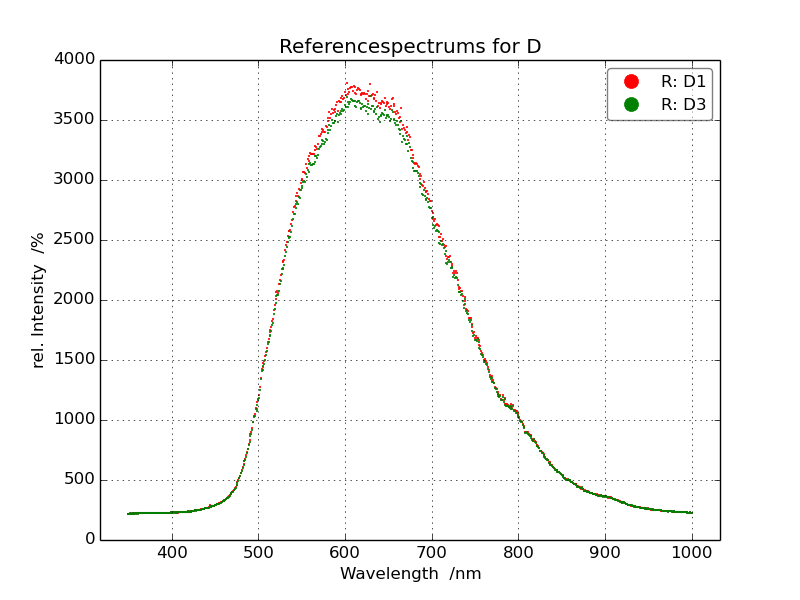
\includegraphics[width=\textwidth]{Figures/Refspec_DPol90.png}
          \caption{Reference spectra for sample-column \textbf{D} at
              $\SI{90}{\degree}$ polarisation.}
          \label{fig:Refspec_DPol90}
        \end{minipage}
      \end{figure}
      \newpage
      \begin{figure}[ht!]
        \centering
        \begin{minipage}{.92\textwidth}
          \centering
          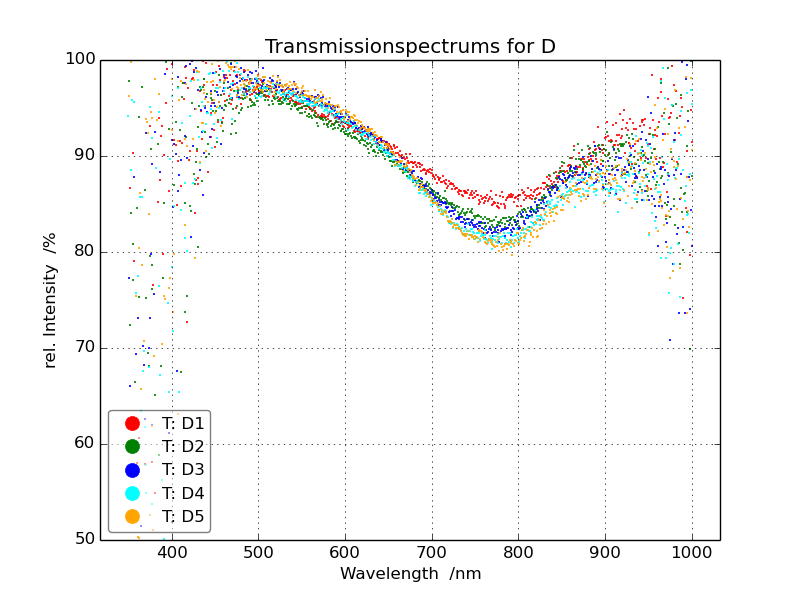
\includegraphics[width=\textwidth]{Figures/TransspecRAW_DPol0.png}
          \caption{Data for sample-column \textbf{D} at $\SI{0}{\degree}$
              polarisation.}
          \label{fig:TransspecRAW_DPol0}
        \end{minipage}\\
        \begin{minipage}{.92\textwidth}
          \centering
          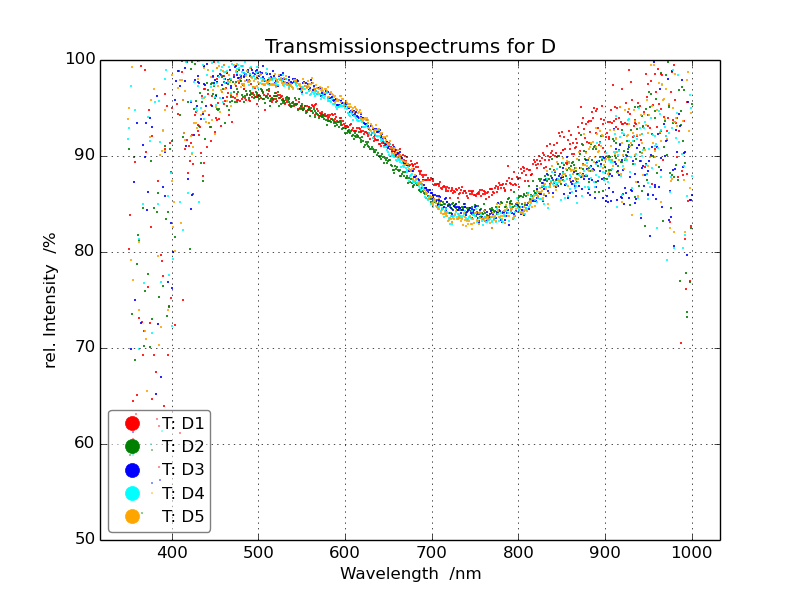
\includegraphics[width=\textwidth]{Figures/TransspecRAW_DPol90.png}
          \caption{Data for sample-column \textbf{D} at $\SI{90}{\degree}$
              polarisation.}
          \label{fig:TransspecRAW_DPol90}
        \end{minipage}
      \end{figure}
      
    \end{section}
    %%%%%%%%%%%%%%%%%%%%%%%%%%%%%%
    
    
    
    \newpage
    %%%%%%%%%%%%%%%%%%%%%%%%%%%%%%
    %%%%%%%%%%%%%%%%%%%%%%%%%%%%%%
    %%%%%%%%%%%%%%%%%%%%%%%%%%%%%%
    \begin{section}{Column \textbf{E}}
      \label{Appendix:DataE}
      
      \begin{figure}[ht!]
        \centering
        \begin{minipage}{.92\textwidth}
          \centering
          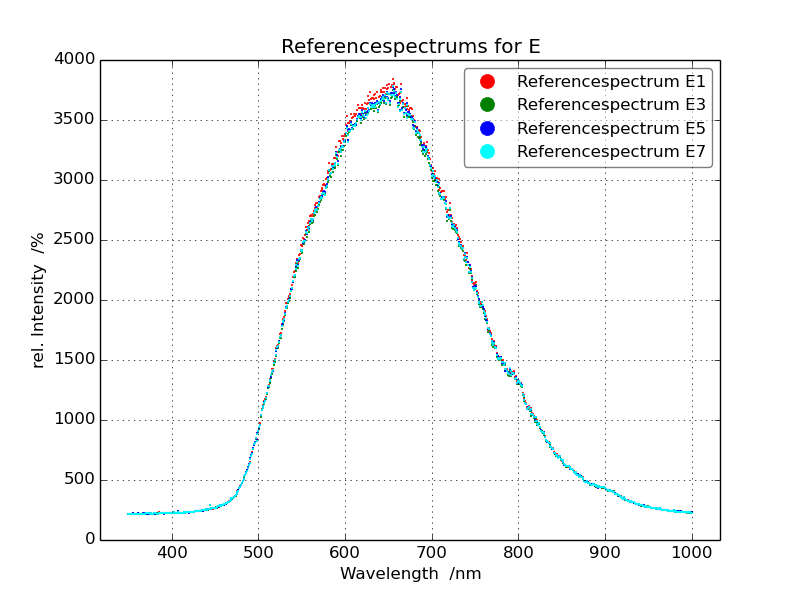
\includegraphics[width=\textwidth]{Figures/Refspec_EPol0.png}
          \caption{Reference spectra for sample-column \textbf{E} at
              $\SI{0}{\degree}$ polarisation.}
          \label{fig:Refspec_EPol0}
        \end{minipage}\\
        \begin{minipage}{.92\textwidth}
          \centering
          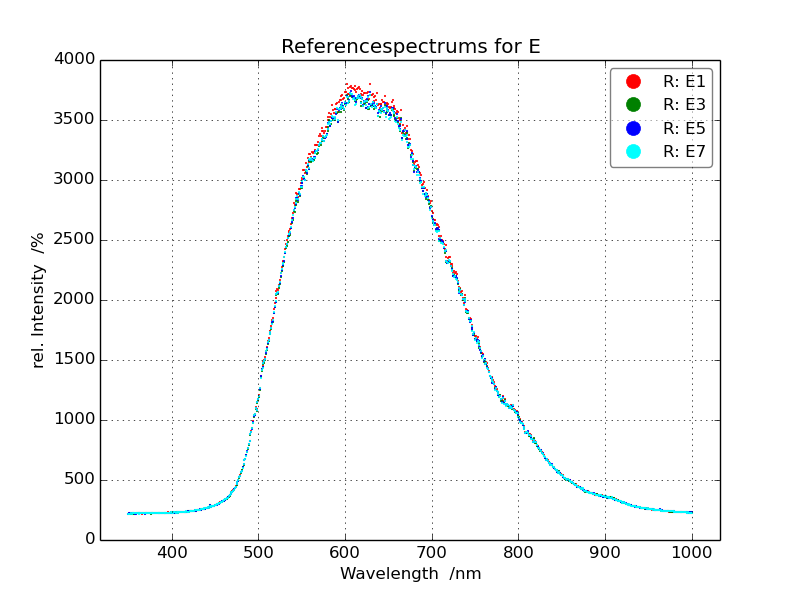
\includegraphics[width=\textwidth]{Figures/Refspec_EPol90.png}
          \caption{Reference spectra for sample-column \textbf{E} at
              $\SI{90}{\degree}$ polarisation.}
          \label{fig:Refspec_EPol90}
        \end{minipage}
      \end{figure}
      \newpage
      \begin{figure}[ht!]
        \centering
        \begin{minipage}{.92\textwidth}
          \centering
          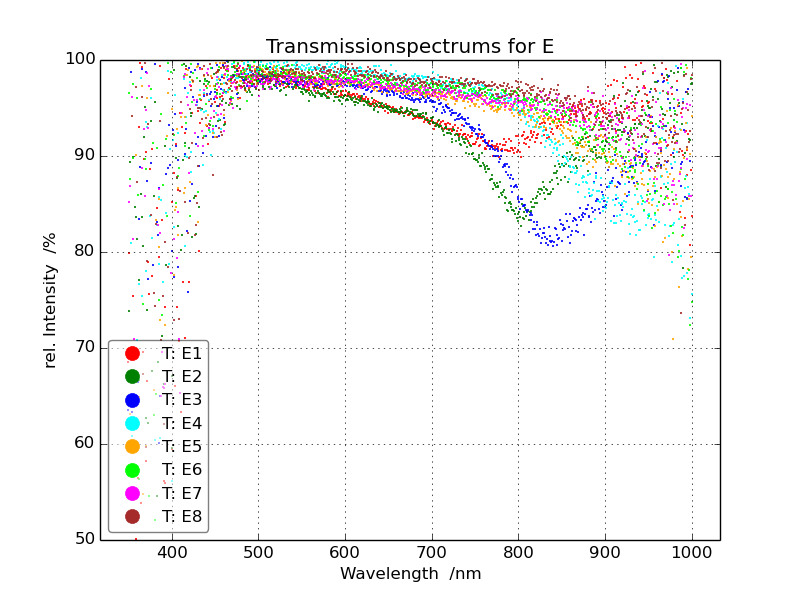
\includegraphics[width=\textwidth]{Figures/TransspecRAW_EPol0.png}
          \caption{Data for sample-column \textbf{E} at $\SI{0}{\degree}$
              polarisation.}
          \label{fig:TransspecRAW_EPol0}
        \end{minipage}\\
        \begin{minipage}{.92\textwidth}
          \centering
          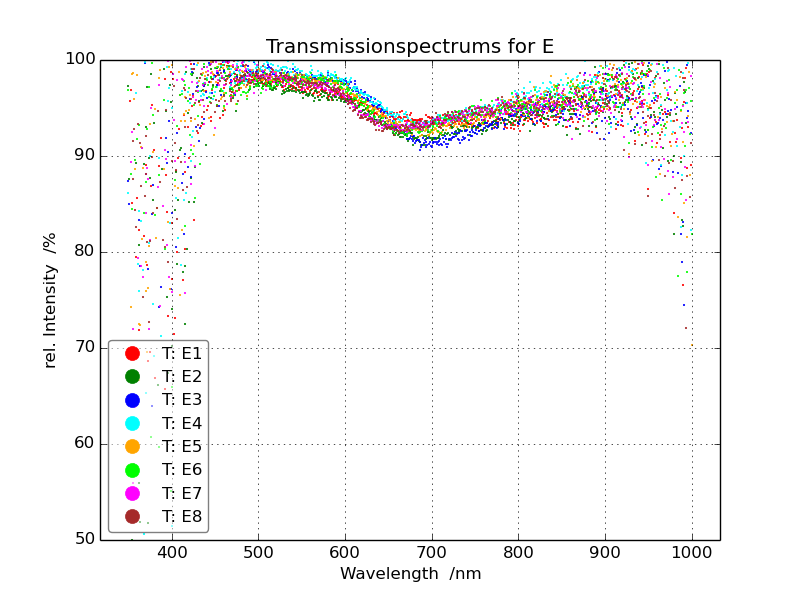
\includegraphics[width=\textwidth]{Figures/TransspecRAW_EPol90.png}
          \caption{Data for sample-column \textbf{E} at $\SI{90}{\degree}$
              polarisation.}
          \label{fig:TransspecRAW_EPol90}
        \end{minipage}
      \end{figure}
      
    \end{section}
    %%%%%%%%%%%%%%%%%%%%%%%%%%%%%%
    
  \end{chapter}
  %%%%%%%%%%%%%%%%%%%%%%%%%%%%%%
  
\end{appendix}
%%%%%%%%%%%%%%%%%%%%
 
  %%%%%%%%%%%%%%%%%%%%
  
  
  
  %%%%%%%%%%%%%%%%%%%%
  %%%%%%%%%%%%%%%%%%%%
  %%%%%%%%%%%%%%%%%%%%
  \begin{thebibliography}{99}
    \scriptsize
    \bibitem{bib:Anleitung}\url{http://www.praktika.physik.uni-bonn.de/module/physik412/downloads/p441d}
\bibitem{bib:}\url{bla}
  \end{thebibliography}
  %%%%%%%%%%%%%%%%%%%%
 
\end{document}
%%%%%%%%%%
